%%%%%%%%%%%%%%%%%%%%%%%%%%%%%%%%%%%%%%%%%%%%%%%%%%%%%%%%%%%%
%%%%%%%%%%%%%%%%%%%%%%% preamble %%%%%%%%%%%%%%%%%%%%%%%%%%%
%%%%%%%%%%%%%%%%%%%%%%%%%%%%%%%%%%%%%%%%%%%%%%%%%%%%%%%%%%%%

\documentclass[compress,red,12pt]{beamer}
\mode<presentation>

%
% Beamer default paper size is 128mm by 96mm
%

\usetheme{Singapore}
% other themes: AnnArbor, Antibes, Bergen, Berkeley, Berlin,
%               Boadilla, boxes, CambridgeUS, Copenhagen,
%               Darmstadt, default, Dresden, Frankfurt, Goettingen,
%               Hannover, Ilmenau, JuanLesPins, Luebeck, Madrid, Maloe,
%               Marburg, Montpellier, PaloAlto, Pittsburg, Rochester,
%               Singapore, Szeged, classic

\usecolortheme{seahorse}
% color themes: albatross, beaver, beetle, crane, default, dolphin, dov,
%               fly, lily, orchid, rose, seagull, seahorse, sidebartab,
%               structure, whale, wolverine

\usefonttheme{structurebold}
% font themes: default, professionalfonts, serif, structurebold,
%               structureitalicserif, structuresmallcapsserif

%
% uncomment to go automatically to full screen
%
%\hypersetup{pdfpagemode=FullScreen}

% define your own colors:
\definecolor{Red}{rgb}{1,0,0}
\definecolor{Blue}{rgb}{0,0,1}
\definecolor{Green}{rgb}{0,1,0}
\definecolor{magenta}{rgb}{1,0,.6}
\definecolor{lightblue}{rgb}{0,.5,1}
\definecolor{lightpurple}{rgb}{.6,.4,1}
\definecolor{gold}{rgb}{.6,.5,0}
\definecolor{orange}{rgb}{1,0.4,0}
\definecolor{hotpink}{rgb}{1,0,0.5}
\definecolor{newcolor2}{rgb}{.5,.3,.5}
\definecolor{newcolor}{rgb}{0,.3,1}
\definecolor{newcolor3}{rgb}{1,0,.35}
\definecolor{darkgreen1}{rgb}{0, .35, 0}
\definecolor{darkgreen}{rgb}{0, .6, 0}
\definecolor{darkred}{rgb}{.75,0,0}

\xdefinecolor{olive}{cmyk}{0.64,0,0.95,0.4}
\xdefinecolor{purpleish}{cmyk}{0.75,0.75,0,0}

% can also choose different themes for the "inside" and "outside"

% \usepackage{beamerinnertheme_______}
% inner themes include circles, default, inmargin, rectangles, rounded
\useinnertheme{circles}

% \usepackage{beamerouterthemesmoothbars}
% outer themes include default, infolines, miniframes, shadow, sidebar,
%               smoothbars, smoothtree, split, tree
%\useoutertheme{miniframes}

% to have the same footer on all slides
%\setbeamertemplate{footline}[text line]{STUFF HERE!}
%\setbeamertemplate{footline}[text line]{} % makes the footer EMPTY
%\setbeamertemplate{footline}{\scriptsize{\vspace*{0.4cm}\hspace*{0.3cm}\insertframenumber}} 
\setbeamertemplate{footline}{\insertpagenumber}

%
% Suppress the navigation symbols
%
\setbeamertemplate{navigation symbols}{}

%
% Make the '\Huge' font size bigger
%
\newcommand\HUGE{\fontsize{60}{70}\selectfont}

%
% Define a title frame
%
\newcommand*\TitleFrame[2]{%
  {%
  \setbeamercolor{background canvas}{bg=purpleish}%
  \begin{frame}[plain]{#1}%
    \begin{center}%
      {\HUGE {#2}}%
    \end{center}%
  \end{frame}%
  }%
}


%
% Automatic Outline
%
\AtBeginSection[section]
{
  \TitleFrame{}{\insertsectionhead}

  \begin{frame}{}
    \begin{center}
      {\huge \insertsectionhead}\\
      ~\\
      \tableofcontents[sectionstyle=hide/hide,subsectionstyle=show/show/hide]
    \end{center}
  \end{frame}
}



%%%%%%%%%%%%%%%%%%%%%%%%%%%%%%%%%%%%%%%%%%%%%%%%%%%%%%%%%%%%
%%%%%%%%%%%%%%%%%%%%%%% Pacakges  %%%%%%%%%%%%%%%%%%%%%%%%%%
%%%%%%%%%%%%%%%%%%%%%%%%%%%%%%%%%%%%%%%%%%%%%%%%%%%%%%%%%%%%

%
% include packages
%
\usepackage[latin1]{inputenc}
\usepackage[small]{caption}
\captionsetup{labelformat=empty, labelsep=none}
\usepackage{animate}
\usepackage{graphicx}
\graphicspath{{./images/}}
\usepackage{bm}
\usepackage{fancybox}
\usepackage{media9}
\usepackage{amsmath}
\usepackage{amssymb}
\usepackage[overlay,absolute]{textpos}
\usepackage{cancel}
\usepackage{color}

\usepackage{tikz}
\usetikzlibrary{shadows.blur}
\usetikzlibrary{arrows,shapes,shapes.callouts,decorations.pathmorphing,backgrounds}
\tikzstyle{every picture}+=[remember picture]
\tikzstyle{na} = [baseline=-.5ex]

\tikzstyle{nodeblue}=[fill=blue!20, anchor=base, rounded corners=2pt]
\tikzstyle{nodered}=[fill=red!20, anchor=base, rounded corners=2pt]
\tikzstyle{nodegreen}=[fill=green!20, anchor=base, rounded corners=2pt]
\tikzstyle{nodeyellow}=[fill=yellow!20, anchor=base, rounded corners=2pt]

\newcommand{\CloudNote}[3]{
  \begin{tikzpicture}[overlay,remember picture, every text node part/.style={align=center}]
    \pgftransformshift{\pgfpointanchor{current page}{center}}
    \node[
    starburst,
    draw=black,
    ultra thick,
    fill=magenta,
    text width=#1,
    align=center,
    anchor=center,
    blur shadow={shadow blur steps=5}
    ] at (#2) {#3};
  \end{tikzpicture}
}

\tikzset{
  invisible/.style={fill=white},
  visible on/.style={alt=#1{}{invisible}},
  alt/.code args={<#1>#2#3}{%
    \alt<#1>{\pgfkeysalso{#2}}{\pgfkeysalso{#3}} % \pgfkeysalso doesn't change the path
  },
}

%%%%%%%%%%%%%%%%%%%%%%%%%%%%%%%%%%%%%%%%%%%%%%%%%%%%%%%%%%%%
%%%%%%%%%%%%%%%%%% Custom Commands I Use  %%%%%%%%%%%%%%%%%%
%%%%%%%%%%%%%%%%%%%%%%%%%%%%%%%%%%%%%%%%%%%%%%%%%%%%%%%%%%%%
\DeclareMathAlphabet\mathbfcal{OMS}{cmsy}{b}{n}
\DeclareMathOperator*{\argmin}{\arg\!\min}

%
% Note:
% Nice curly font is {\bm{\mathcal{D}}}
%
\newcommand{\Grad}[1]{\bm{\triangledown_{#1}}}
\newcommand{\abbrev}[1]{\rm{#1}}
%\newcommand{\argmin}{\mathrm{arg}\min}
\newcommand{\curly}[1]{\left\{#1\right\}}
\newcommand{\roundy}[1]{\left(#1\right)}
\newcommand{\recty}[1]{\left[#1\right]}
\newcommand{\PartDeriv}[2]{\frac{\partial{#1}}{\partial{#2}}}
\newcommand{\vect}[1]{\bm{#1}}
\newcommand{\mat}[1]{\bm{#1}}
\newcommand{\transpose}[1]{{#1}^\intercal}
\newcommand{\derivsym}[1]{\,d{#1}}

%
% Used symbols (only partial for now...)
%
\newcommand{\OpSphere}{\mathbfcal{S}}
\newcommand{\OpRot}{\mathbfcal{R}}
\newcommand{\OpDistance}{\bm{D}}
\newcommand{\OpCumsum}{\mathbfcal{C}}
\newcommand{\OpInt}{\mathbfcal{I}}
\newcommand{\OpCamera}{\mathbfcal{P}}
\newcommand{\MaskSun}{\mathbfcal{M}}
\newcommand{\Laplacian}{\mathbfcal{L}}
\newcommand{\OpDiag}[1]{\mathbb{D}\left\{#1\right\}}
\newcommand{\DistSet}{\mathcal{C}}
\newcommand{\DistUnknown}{\vect{n}}
\newcommand{\DistEstimated}{\hat{\vect{n}}}
\newcommand{\CostFunc}[1]{E(#1)}



%
% To speed up of compilation
%
%\includeonlyframes{current}

%%%%%%%%%%%%%%%%%%%%%%%%%%%%%%%%%%%%%%%%%%%%%%%%%%%%%%%%%%%%
%%%%%%%%%%%%%%%%%% title page information %%%%%%%%%%%%%%%%%%
%%%%%%%%%%%%%%%%%%%%%%%%%%%%%%%%%%%%%%%%%%%%%%%%%%%%%%%%%%%%

\title[3D Aerosol Recovery]{
  Lightfield Analysis and Recovery of the Atmosphere
}

\author[Amit Aides]{
  Amit Aides \\
  Supervisor: Prof. Yoav Y. Schechner
}

\date{12 September 2013}

%%%%%%%%%%%%%%%%%%%%%%%%%%%%%%%%%%%%%%%%%%%%%%%%%%%%%%%%%%%%
%%%%%%%%%%%%%%%%%%%%%%% begin %%%%%%%%%%%%%%%%%%%%%%%%%%%%%%
%%%%%%%%%%%%%%%%%%%%%%%%%%%%%%%%%%%%%%%%%%%%%%%%%%%%%%%%%%%%

\begin{document}

\begin{frame}
  \titlepage
\end{frame}

%%%%%%%%%%%%%%%%%%%%%%%%%%%%%%%%%%%%%%%%%%%%%%%%%%%%%%%%%%%%
%%%%%%%%%%%%%%%%%%%%%%%%%%%%%%%%%%%%%%%%%%%%%%%%%%%%%%%%%%%%
%%%%%%%%%%%%%%%%%%%%%%%%%%%%%%%%%%%%%%%%%%%%%%%%%%%%%%%%%%%%

\section{Introduction}

%%%%%%%%%%%%%%%%%%%%%%%%%%%%%%%%%%%%%%%%%%%%
%%%%%%%%%%%%%%%%%%%%%%%%%%%%%%%%%%%%%%%%%%%%
%%%%%%%%%%%%%%%%%%%%%%%%%%%%%%%%%%%%%%%%%%%%

\subsection{Motivation}

\begin{frame}[label=motivation]{Aerosols in the Atmosphere}
  \begin{center}
    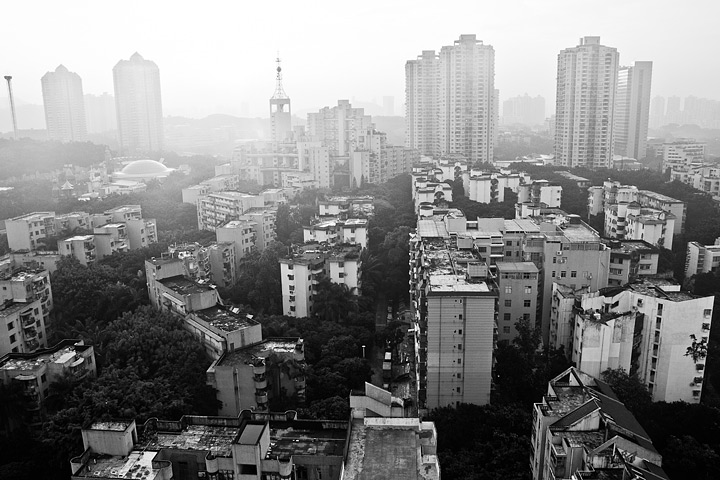
\includegraphics[height=7cm]{images/shenzen_haze.jpg}
  \end{center}    
  \begin{center}
    \hyperlink{aerosols-data}{\beamergotobutton{Aerosols Info}}\hfill
    {\tiny http://earthobservatory.nasa.gov/Features/Aerosols/}
  \end{center}
\end{frame}

%%%%%%%%%%%%%%%%%%%%%%%%%%%%%%%%%%%%%%%%%%%%%%%%%%%%%%%

\begin{frame}{Eyjafjallaj\"{o}kull Eruption in 2010}
  \begin{center}
    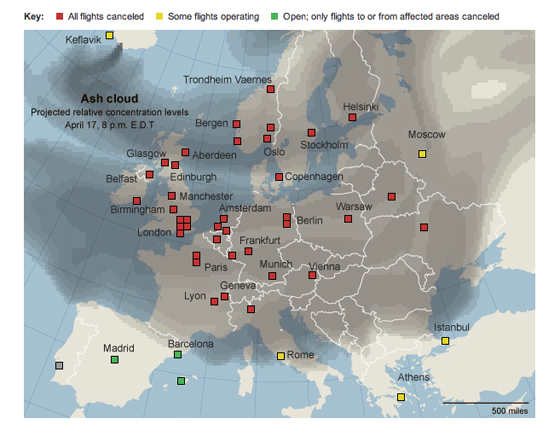
\includegraphics[height=7cm]{images/volcano-airport.jpg}
  \end{center}
  \begin{flushright}
    \includemedia[
    addresource=sounds/mountain_name.mp3,
    flashvars={
      source=sounds/mountain_name.mp3
      &autoPlay=false
    }
    ]{\fbox{Play}}{APlayer.swf}
    {\tiny http://www.metrolic.com/eyjafjallajokull-is-dormant...for-the-moment-2042/}
  \end{flushright}
\end{frame}

%%%%%%%%%%%%%%%%%%%%%%%%%%%%%%%%%%%%%%%%%%%%
%%%%%%%%%%%%%%%%%%%%%%%%%%%%%%%%%%%%%%%%%%%%
%%%%%%%%%%%%%%%%%%%%%%%%%%%%%%%%%%%%%%%%%%%%

\subsection{PhD Task}

\begin{frame}{Multi-angle Tomographic Reconstruction}
  \begin{center}
    \only<1>
    {
      \centerline{\def\svgwidth{\linewidth}\small{\input{images/camera_network1.pdf_tex}}}
    }
    \only<2>
    {
      \centerline{\def\svgwidth{\linewidth}\small{\input{images/camera_network2.pdf_tex}}}
    }
  \end{center}
\end{frame}

%%%%%%%%%%%%%%%%%%%%%%%%%%%%%%%%%%%%%%%%%%%%%%%%%%%%%%%

\begin{frame}{Multi-angle imaging from the ground}
  \begin{columns}[T]
    \begin{column}{.5\textwidth}
      \begin{itemize}
      \item 3D reconstruction
      \item Simple setup
      \item Based on Sun light scattering and attenuation
      \end{itemize}
    \end{column}
    \begin{column}{.5\textwidth}
      \centering
      {\includegraphics[height=3cm]{images/camera_network-1.png}}
    \end{column}
  \end{columns}
\end{frame}

%%%%%%%%%%%%%%%%%%%%%%%%%%%%%%%%%%%%%%%%%%%%%%%%%%%%%%%

\begin{frame}{Simulated Reconstruction}
  \begin{center}
    \only<1>{
      \animategraphics[width=0.9\linewidth, loop, controls, buttonsize=5pt]{3}{images/result_movie1/snapshot1_}{0}{35}
    }
    \only<2>{
      \animategraphics[width=0.9\linewidth, loop, controls, buttonsize=5pt]{3}{images/result_movie1/snapshot2_}{0}{35}
    }
  \end{center}
  \begin{center}
    \tiny{Color represents aerosol density. The density units are $10^{6}~{\rm particles}/{\rm m}^3$}
  \end{center}
\end{frame}

%%%%%%%%%%%%%%%%%%%%%%%%%%%%%%%%%%%%%%%%%%%%%%%%%%%%%%%

\begin{frame}{}
  \includemedia[
  label=video1,
  width=1.0\linewidth,height=0.66\linewidth,
  activate=pageopen,
  addresource=videos/cloudsnew.mp4,
  flashvars={source=videos/cloudsnew.mp4}
  ]{}{VPlayer.swf}
\end{frame}

%%%%%%%%%%%%%%%%%%%%%%%%%%%%%%%%%%%%%%%%%%%%%%%%%%%%%%%

\begin{frame}{}
  \begin{center}
    \begin{block}{Publications}
      \begin{itemize}
      \item Presented in the MISR Data Users Science Symposium Dec. 2012, Pasadena, CA, USA
      \item In review, Optics Express.
      \end{itemize}
    \end{block}
  \end{center}
\end{frame}

%%%%%%%%%%%%%%%%%%%%%%%%%%%%%%%%%%%%%%%%%%%%
%%%%%%%%%%%%%%%%%%%%%%%%%%%%%%%%%%%%%%%%%%%%
%%%%%%%%%%%%%%%%%%%%%%%%%%%%%%%%%%%%%%%%%%%%

\subsection{State of The Art}

\TitleFrame{}{State of The Art}

\begin{frame}{Remote Sensing}
  \begin{center}
    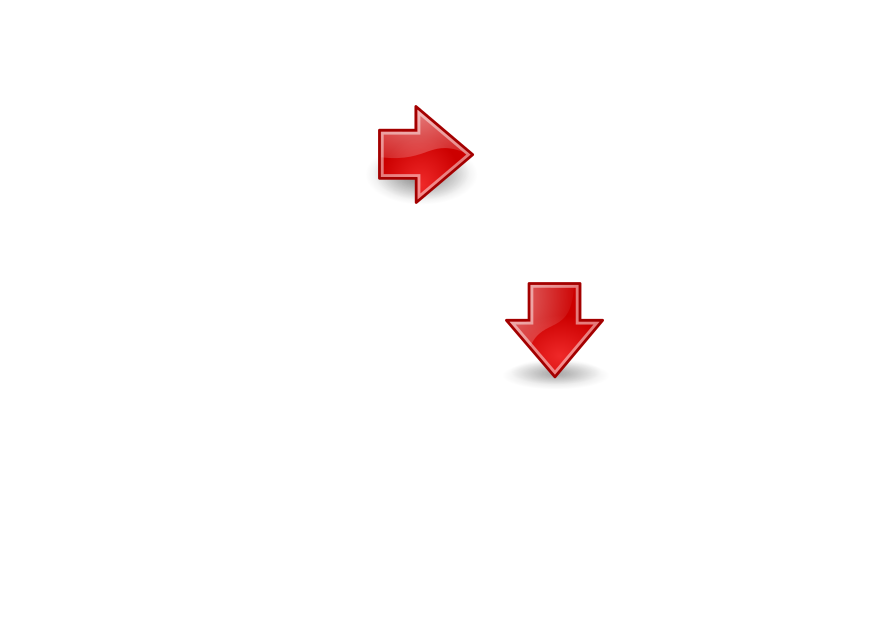
\includegraphics[width=0.9\textwidth]{images/misr.pdf}
  \end{center}
  \begin{flushright}
    {\tiny http://earthobservatory.nasa.gov/}
  \end{flushright}
  \only<2>
  {
    \CloudNote{0.4\textwidth}{0, 0}{
      Low resolution \\
      2D reconstruction \\
      Top viewing point \\
      Expensive}
  }
\end{frame}

%%%%%%%%%%%%%%%%%%%%%%%%%%%%%%%%%%%%%%%%%%%%%%%%%%%%%%%

\begin{frame}{LIDAR - Light Detection And Ranging}
  \begin{center}
    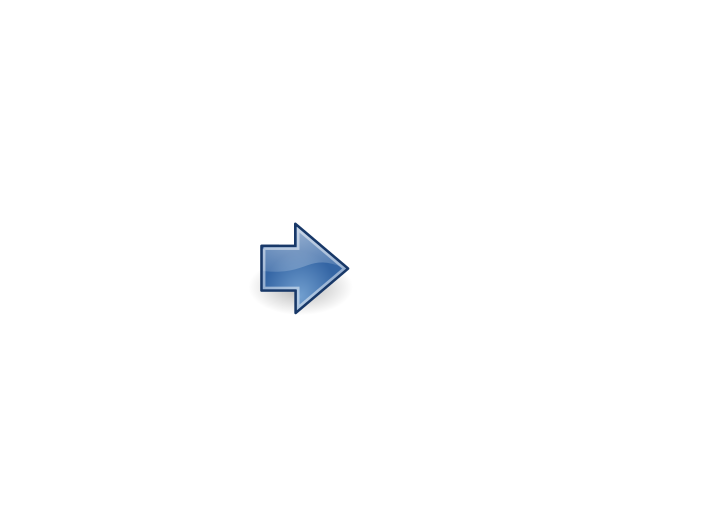
\includegraphics[width=0.9\columnwidth]{images/lidar.pdf}
  \end{center}

  \begin{flushright}
    {\tiny http://jp.hamamatsu.com/en/rd/technology/energy/lidar.html}
    %\only<2> {\tiny http://earthobservatory.nasa.gov/}
  \end{flushright}
  \only<2>
  {
    \CloudNote{0.4\textwidth}{0, 0}{
      Local \\
      Expensive}
  }
\end{frame}

%%%%%%%%%%%%%%%%%%%%%%%%%%%%%%%%%%%%%%%%%%%%%%%%%%%%%%%
%%%%%%%%%%%%%%%%%%%%%%%%%%%%%%%%%%%%%%%%%%%%%%%%%%%%%%%
%%%%%%%%%%%%%%%%%%%%%%%%%%%%%%%%%%%%%%%%%%%%%%%%%%%%%%%

\section{Theory}

%%%%%%%%%%%%%%%%%%%%%%%%%%%%%%%%%%%%%%%%%%%%
%%%%%%%%%%%%%%%%%%%%%%%%%%%%%%%%%%%%%%%%%%%%
%%%%%%%%%%%%%%%%%%%%%%%%%%%%%%%%%%%%%%%%%%%%

\subsection{Radiative Transfer}

\begin{frame}[label=RT]{Radiation Transfer}
  Light interaction with the atmosphere:
  \begin{itemize}
  \item Loses energy to absorption
  \item Gains energy by emission
  \item Redistributes energy by scattering
  \end{itemize}
  \hfill\hyperlink{RTE}{\beamergotobutton{RTE}}  
\end{frame}

%%%%%%%%%%%%%%%%%%%%%%%%%%%%%%%%%%%%%%%%%%%%%%%%%%%%%%%

\begin{frame}{Attenuation}
  \begin{block}{Light is attenuated according to {\em Beer-Lambert} law}
    \centerline{\def\svgwidth{0.6\columnwidth}\small{\input{images/beer_lambert.pdf_tex}}}
  \end{block}
  \begin{tikzpicture}[overlay]
    \onslide<2->
    {
      \node[nodeblue] at (4,0)(s1) {Cross Section};
      \path[->] (s1) edge [bend right] (d1);
    }
    \onslide<3->
    {
      \node[nodered] at (7,-0.5)(s2) {Density};
      \path[->] (s2) edge [bend right] (d2);
    }
  \end{tikzpicture}
  \onslide<4>
  {
    \begin{block}{Optical Depth}
      \begin{align*}
        \tau = \int \sigma n \derivsym{x} \qquad\Longrightarrow\qquad I=I_0 \exp(-\tau)
      \end{align*}
      Measures transparency of medium
    \end{block}
  }
\end{frame}

%%%%%%%%%%%%%%%%%%%%%%%%%%%%%%%%%%%%%%%%%%%%%%%%%%%%%%%

\begin{frame}{Scattering}
    \begin{overprint}
      \only<1>
      {
        \centerline{\def\svgwidth{0.6\linewidth}\small{\input{images/phase_function1.pdf_tex}}}
      }
      \only<2>
      {
        \centerline{\def\svgwidth{0.6\linewidth}\small{\input{images/phase_function2.pdf_tex}}}
      }
      \only<3->
      {
        \centerline{\def\svgwidth{0.6\linewidth}\small{\input{images/phase_function3.pdf_tex}}}
      }
    \end{overprint}
    \onslide<4>
    {
      \begin{center}{Scattering Ratio}
        \begin{align*}
          \alpha = \tikz[baseline]{ \node[nodeyellow] (d1) {$k$}; } \sigma P(\theta) \derivsym{\theta}
        \end{align*}
      \end{center}
      \begin{tikzpicture}[overlay]
        \node[nodeyellow] at (2,.5) (s1) {Albedo};
        \path[->] (s1) edge [bend right] (d1);
      \end{tikzpicture}
    }

\end{frame}

%%%%%%%%%%%%%%%%%%%%%%%%%%%%%%%%%%%%%%%%%%%%%%%%%%%%%%%

\begin{frame}[T]{Phase Functions Used}
  \begin{columns}[T]
    \column{0.6\textwidth}
    \begin{itemize}
    \item Rayleigh scattering - for air molecules
    \item Henyey-Greenstein equation - for aerosols
    \end{itemize}
    \column{0.4\textwidth}
    \centering
    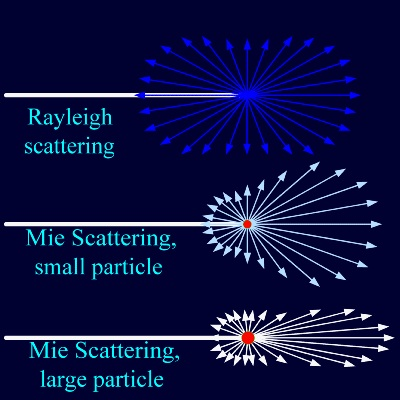
\includegraphics[height=4cm]{images/Mie_Rayleigh.jpg}
  \end{columns}
\end{frame}

%%%%%%%%%%%%%%%%%%%%%%%%%%%%%%%%%%%%%%%%%%%%%%%%%%%%%%%%%%%%
%%%%%%%%%%%%%%%%%%%%%%%%%%%%%%%%%%%%%%%%%%%%%%%%%%%%%%%%%%%%

\section{Ongoing PhD Research}

%%%%%%%%%%%%%%%%%%%%%%%%%%%%%%%%%%%%%%%%%%%%%%%%%%%%%%%

\subsection{overview}

\begin{frame}{}
  \begin{center}
    \includegraphics<1>[height=8cm]{images/diagram.pdf}    
    \includegraphics<2>[height=8cm]{images/diagram_reference_images.pdf}    
    \includegraphics<3>[height=8cm]{images/diagram_models.pdf}    
  \end{center}
\end{frame}

%%%%%%%%%%%%%%%%%%%%%%%%%%%%%%%%%%%%%%%%%%%%%%%%%%%%%%%

\subsection{Single-scattering model}

\begin{frame}{Single-Scattering Model}
  \begin{columns}[C]
    \column{0.4\textwidth}
    \begin{itemize}
    \item Simple
    \item Fast
    \item Analytic
    \end{itemize}

    \column{0.6\textwidth}
    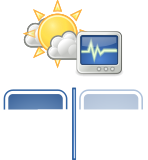
\includegraphics[width=\columnwidth]{images/diagram_models_single.pdf}

  \end{columns}
\end{frame}

%%%%%%%%%%%%%%%%%%%%%%%%%%%%%%%%%%%%%%%%%%%%%%%%%%%%%%%

\begin{frame}{Single-Scattering Model}
  \begin{columns}[c]
    \column{0.5\columnwidth}
    \setbeamercovered{transparent}
    \begin{itemize}
    \item <1-2> Atmosphere volume
    \item <2-3> Voxel - Volume Element
    \item <3> Contains air and aerosols
    \item <4> Light is attenuated due to scattering and absorption
    \item <5> Light scatters only once between source and viewer
    \item <6> Light is attenuated due to scattering and absorption
    \item <7> Simple Analytic model
    \item <7> No Multi-Scattering
    \end{itemize}

    \column{0.5\columnwidth}
    \begin{overlayarea}{\columnwidth}{8cm}
      \only<1> {\centerline{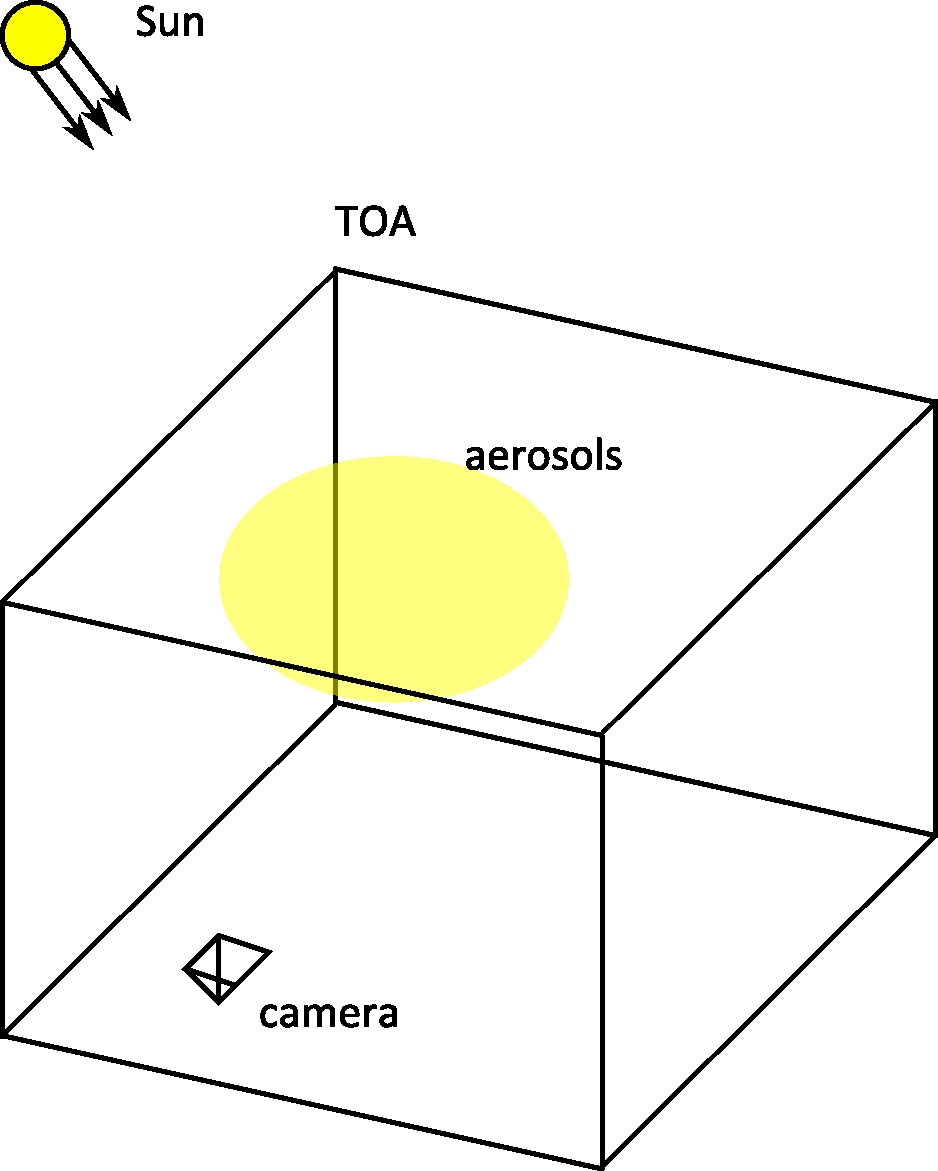
\includegraphics[width=\columnwidth]
          {images/atmo_settings3D1.pdf}}}
      \only<2> {\centerline{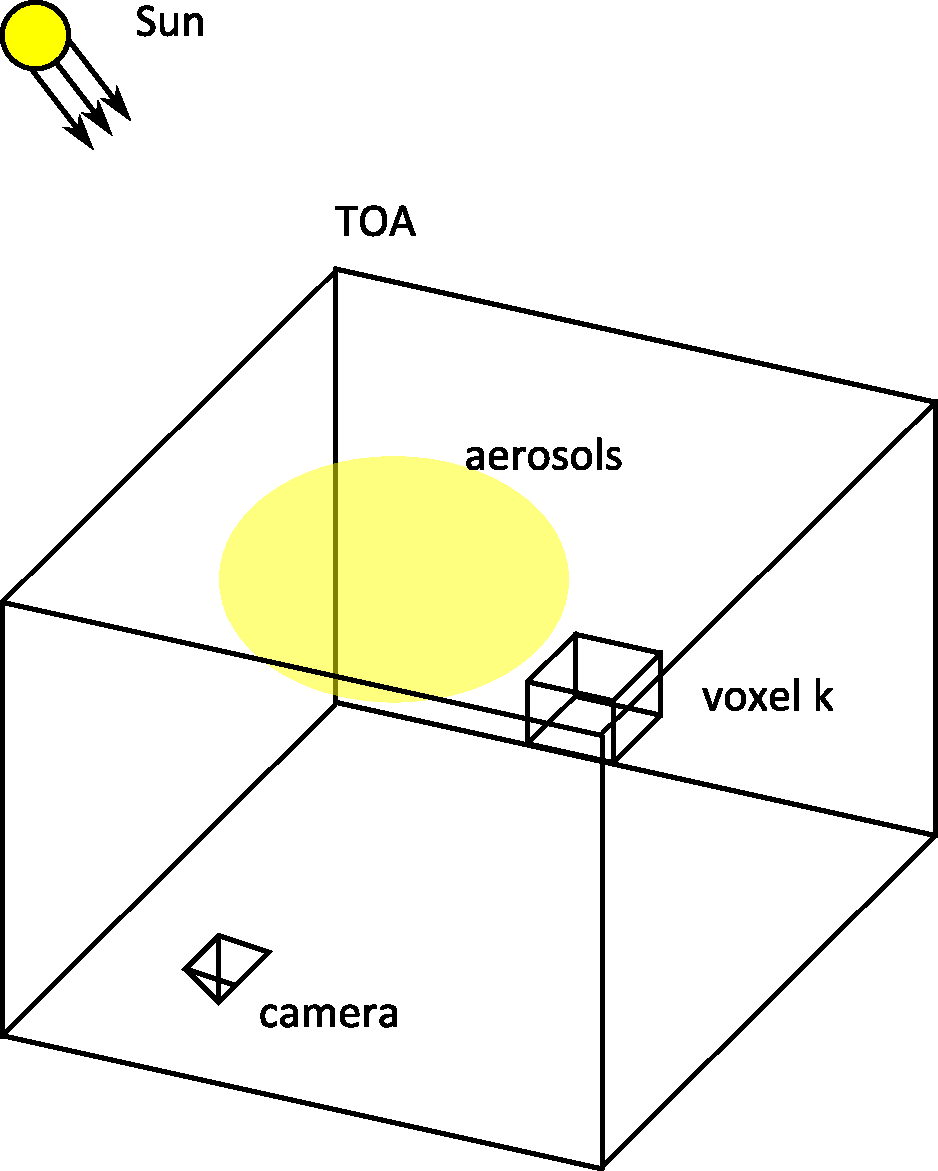
\includegraphics[width=\columnwidth]
          {images/atmo_settings3D2.pdf}}}
      \only<3> {\centerline{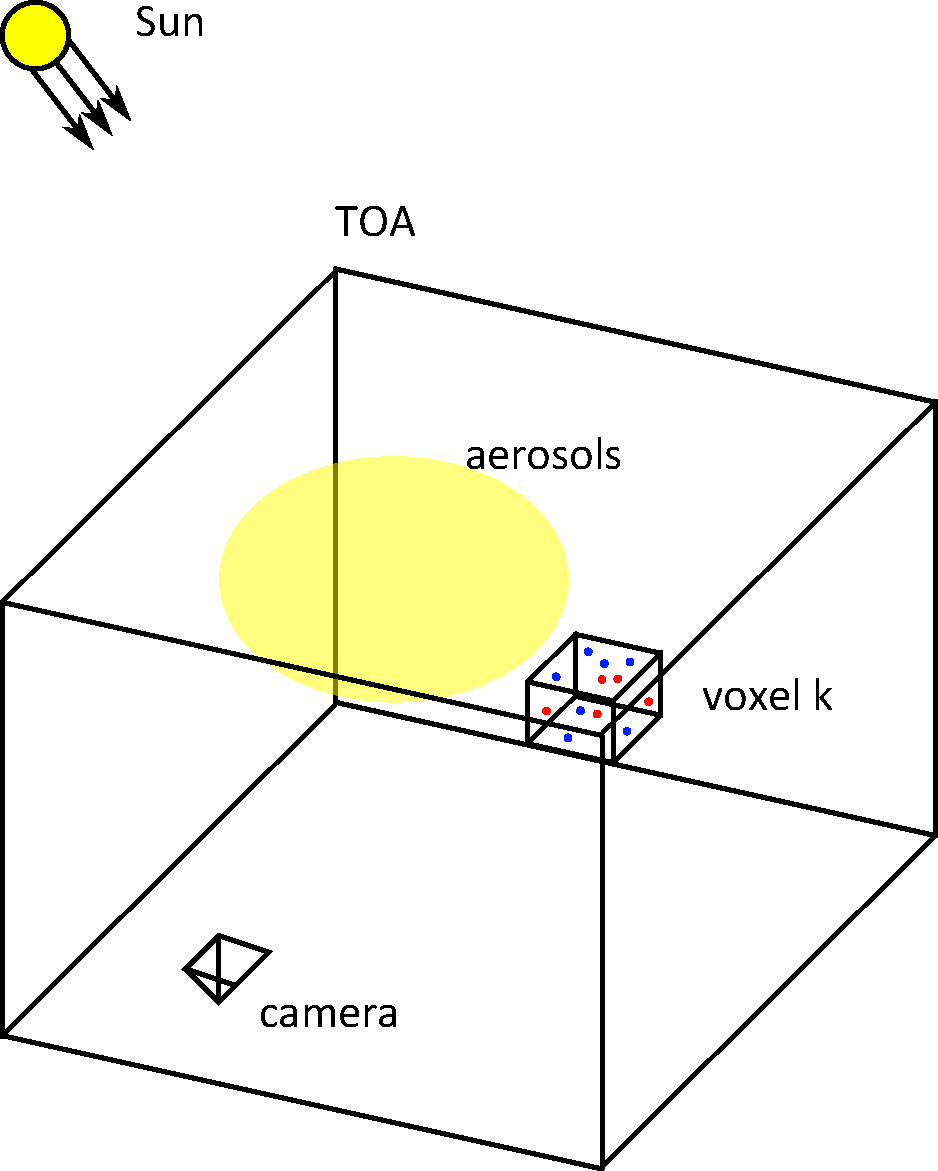
\includegraphics[width=\columnwidth]
          {images/atmo_settings3D3.pdf}}}
      \only<4> {\centerline{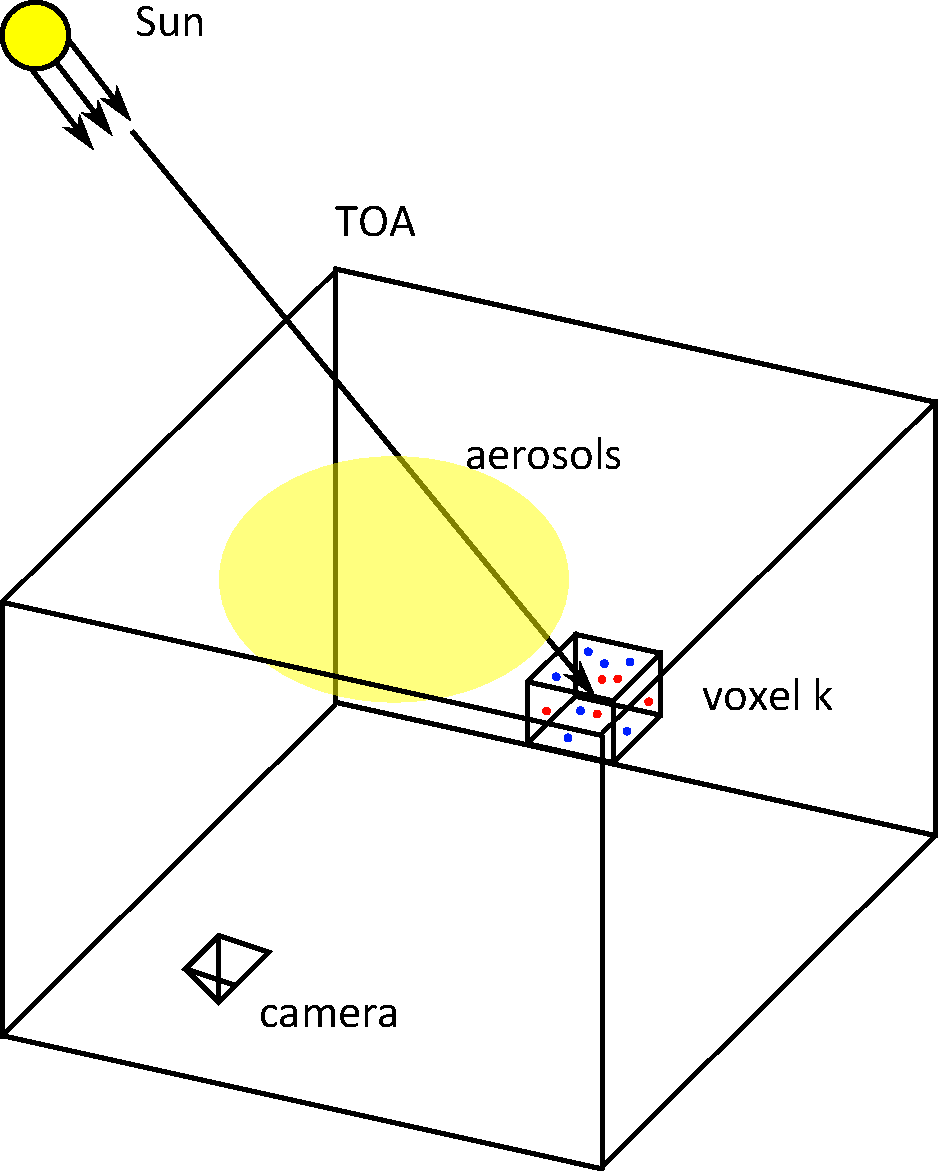
\includegraphics[width=\columnwidth]
          {images/atmo_settings3D4.pdf}}}
      \only<5> {\centerline{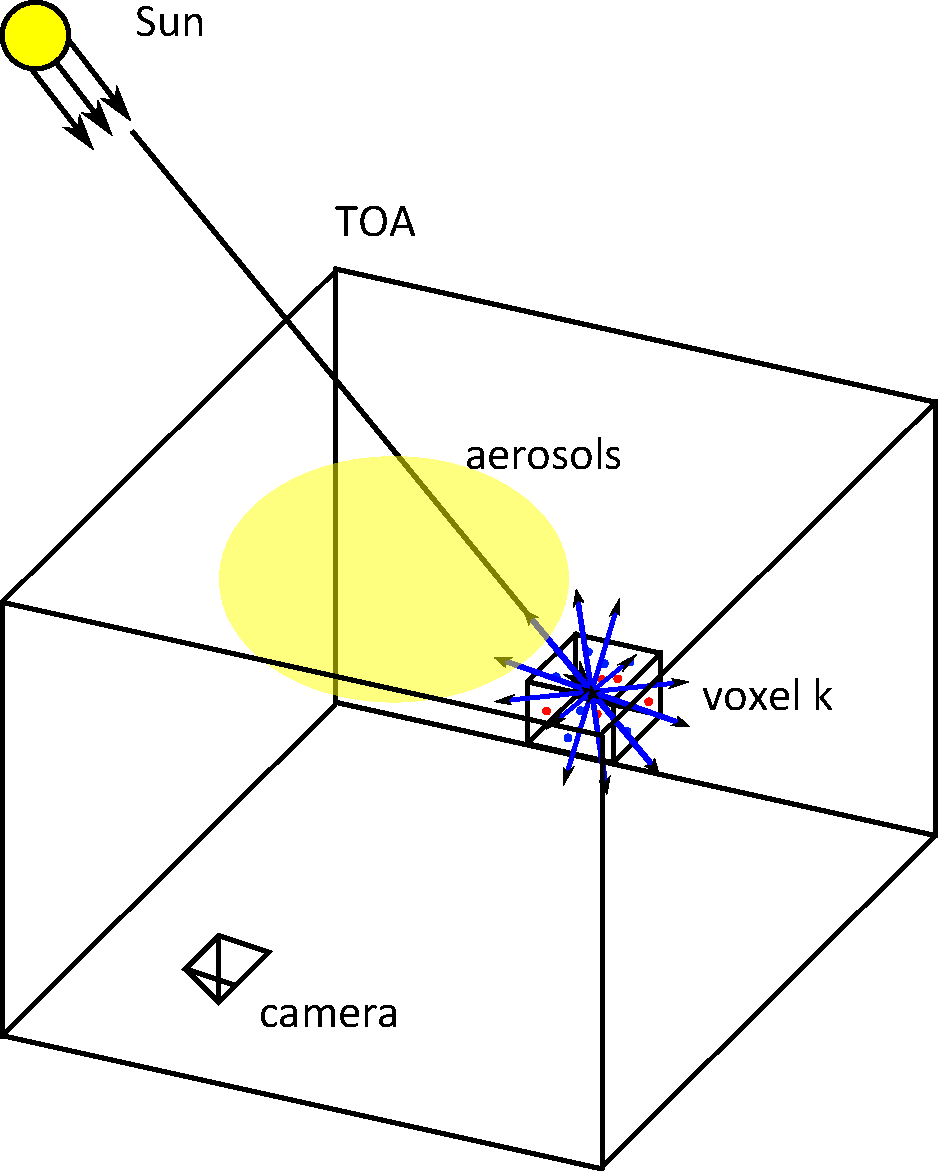
\includegraphics[width=\columnwidth]
          {images/atmo_settings3D5.pdf}}}
      \only<6> {\centerline{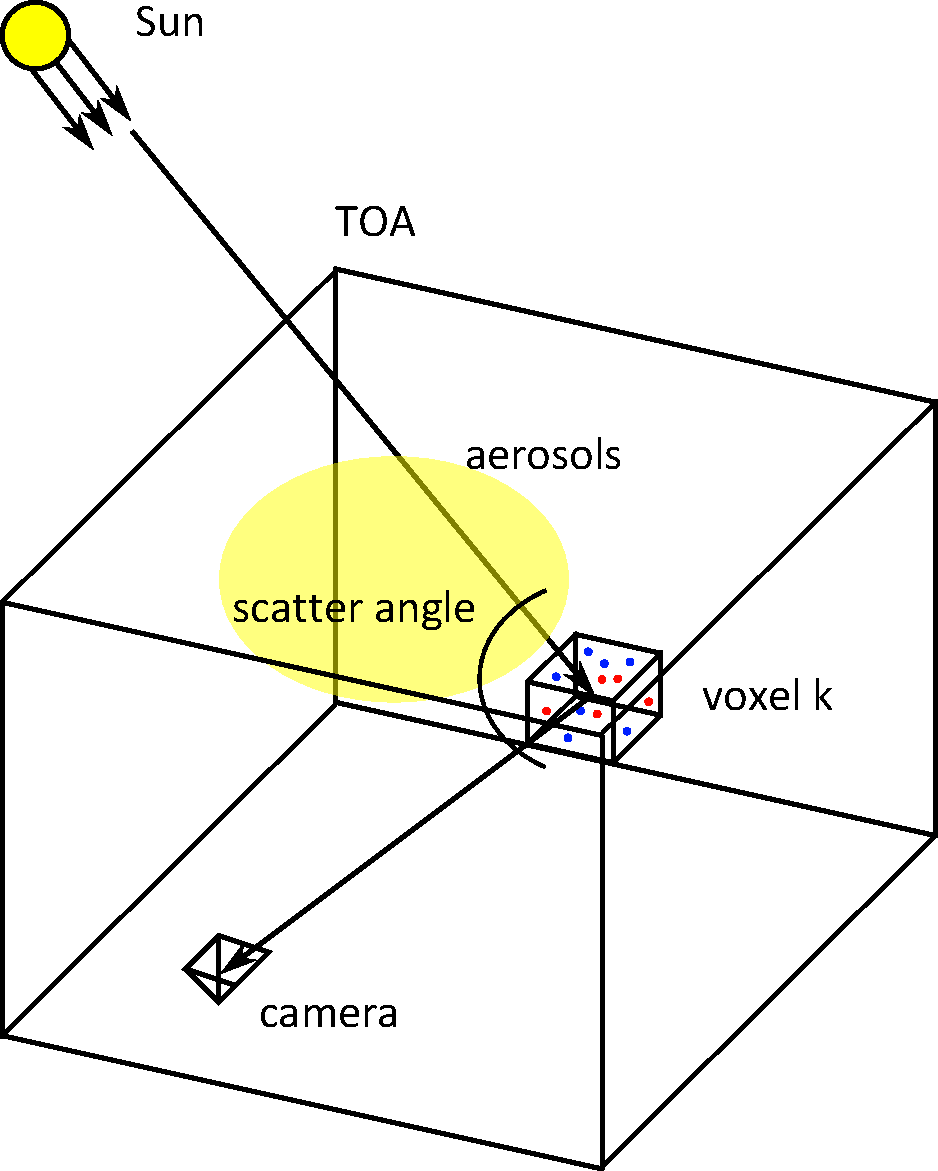
\includegraphics[width=\columnwidth]
          {images/atmo_settings3D6.pdf}}}
      \only<7> {\centerline{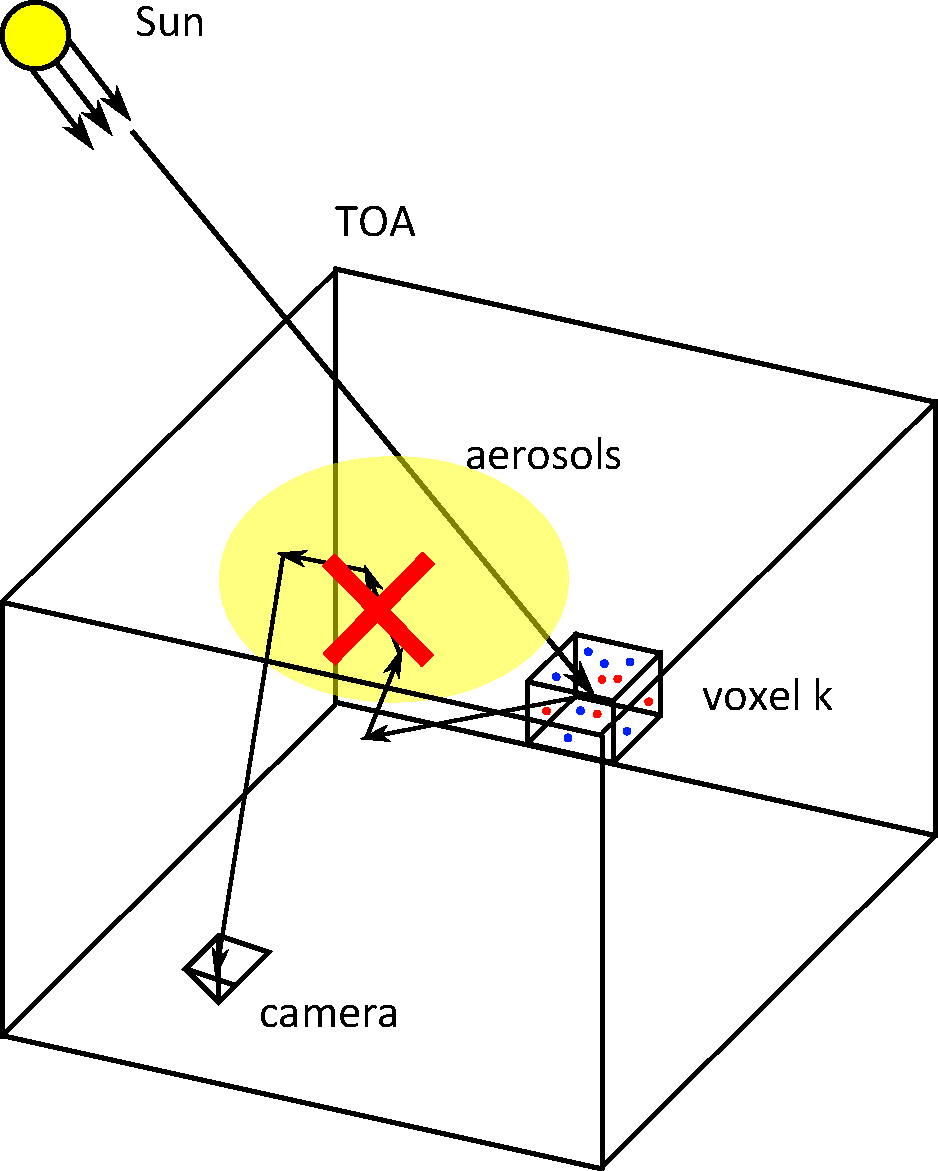
\includegraphics[width=\columnwidth]
          {images/atmo_settings3D7.pdf}}}
    \end{overlayarea}
  \end{columns}
\end{frame}

%%%%%%%%%%%%%%%%%%%%%%%%%%%%%%%%%%%%%%%%%%%%%%%%%%%%%%%

\begin{frame}[label=formation-model]{Image Formation Model}
  \begin{columns}[c]

    \column{0.7\textwidth}
    \begin{itemize}
    \item <3-> Attenuation \tikz[na] \node[coordinate] (s2) {};
    \item <4-> Scattering \tikz[na] \node[coordinate] (s3) {};
    \end{itemize}

    % \small
    \footnotesize
    \begin{align*}
      \mathrm{I} &= \\
      & \tikz[baseline]{ \node[nodeblue, visible on=<2->] (d1) {\hyperlink{TOA}{$\mathrm{L}^{\rm TOA}$}}; } \,
      \tikz[baseline]{ \node[nodered, visible on=<5->] (d4) {$\OpCamera$}; }
      \curly{\roundy{
          \tikz[baseline]{ \node[nodegreen, visible on=<4->] (d3) {$\vect{\alpha}^{\rm aerosol} + \vect{\alpha}^{\rm air}$}; } }  \odot 
        \tikz[baseline]{ \node[nodeyellow, visible on=<3->] (d2) {$\exp^{-(\vect{\tau}^{\rm aerosol} + \vect{\tau}^{\rm air})}$}; } }
    \end{align*}
    \normalsize

    \begin{itemize}
    \item <2-> Sun \tikz[na] \node[coordinate] (s1) {}; luminance 
    \item <5-> Camera projection \tikz[na] \node[coordinate] (s4) {};
    \end{itemize}

    \begin{tikzpicture}[overlay]
      \onslide<2->{\path[->] (s1) edge [bend right] (d1);}
      \onslide<3->{\path[->] (s2) edge [bend left] (d2);}
      \onslide<4->{\path[->] (s3) edge [bend left] (d3);}
      \onslide<5->{\path[->] (s4) edge [bend right] (d4);}
    \end{tikzpicture}

    \column{0.3\textwidth}
    \begin{overprint}
      \only<1-2> {\centerline{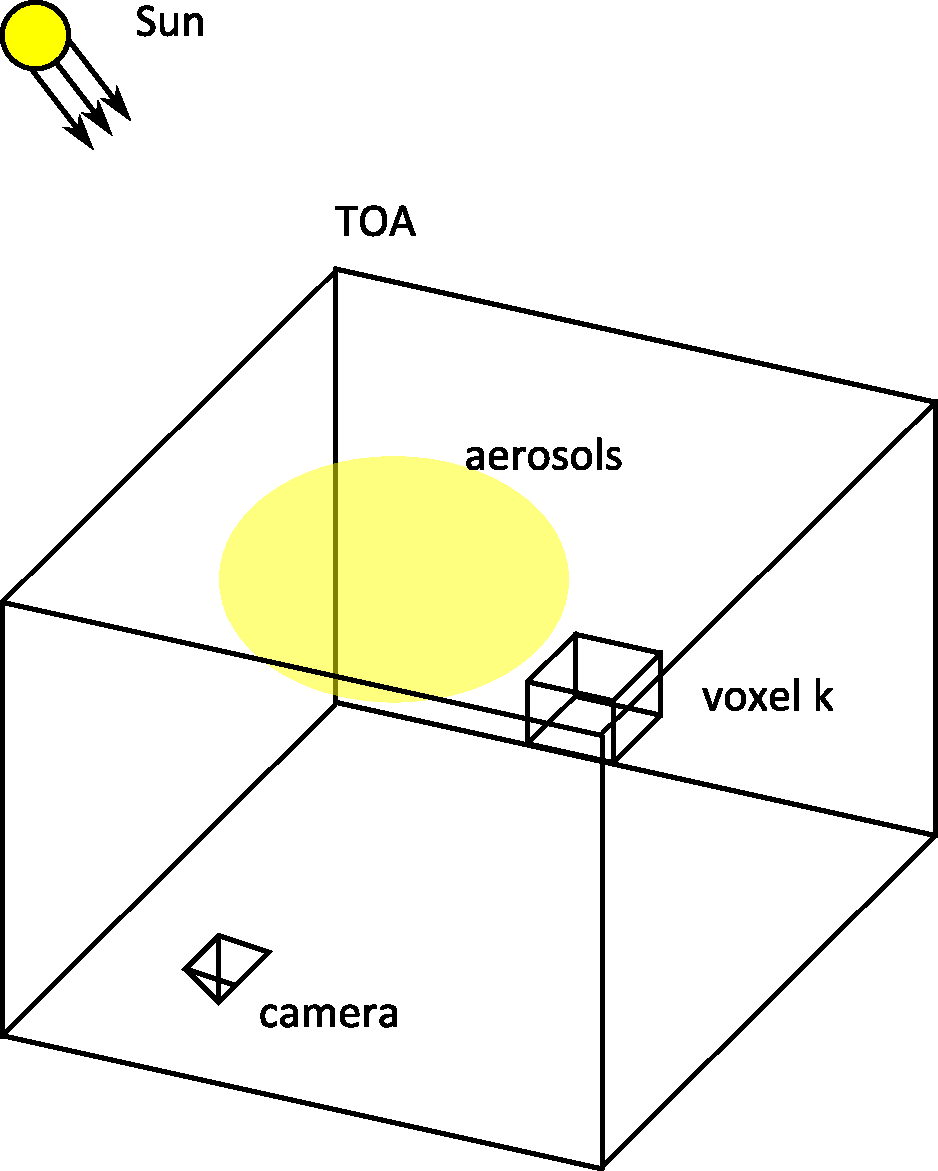
\includegraphics[width=\columnwidth]
          {images/atmo_settings3D2.pdf}}}
      \only<3> {\centerline{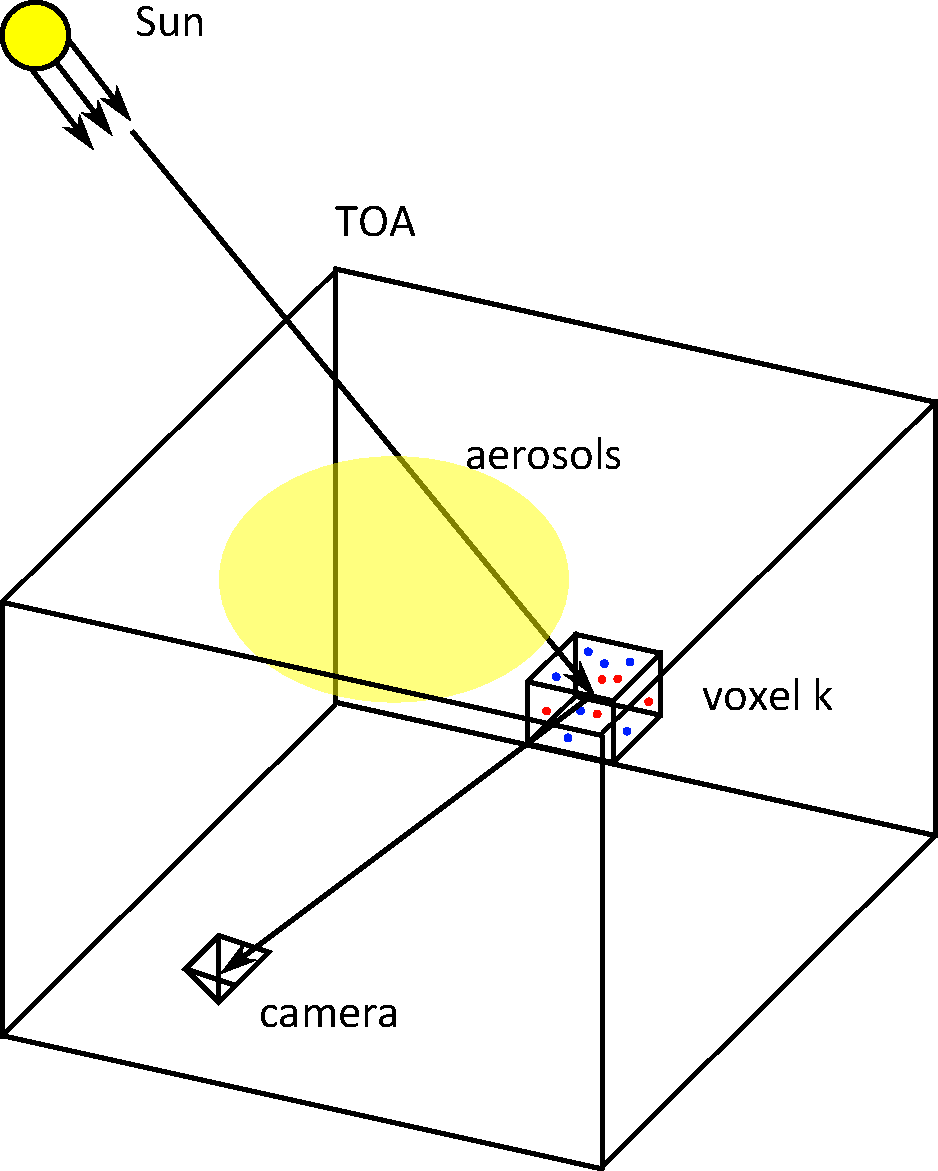
\includegraphics[width=\columnwidth]
          {images/atmo_settings3D10.pdf}}}
      \only<4-> {\centerline{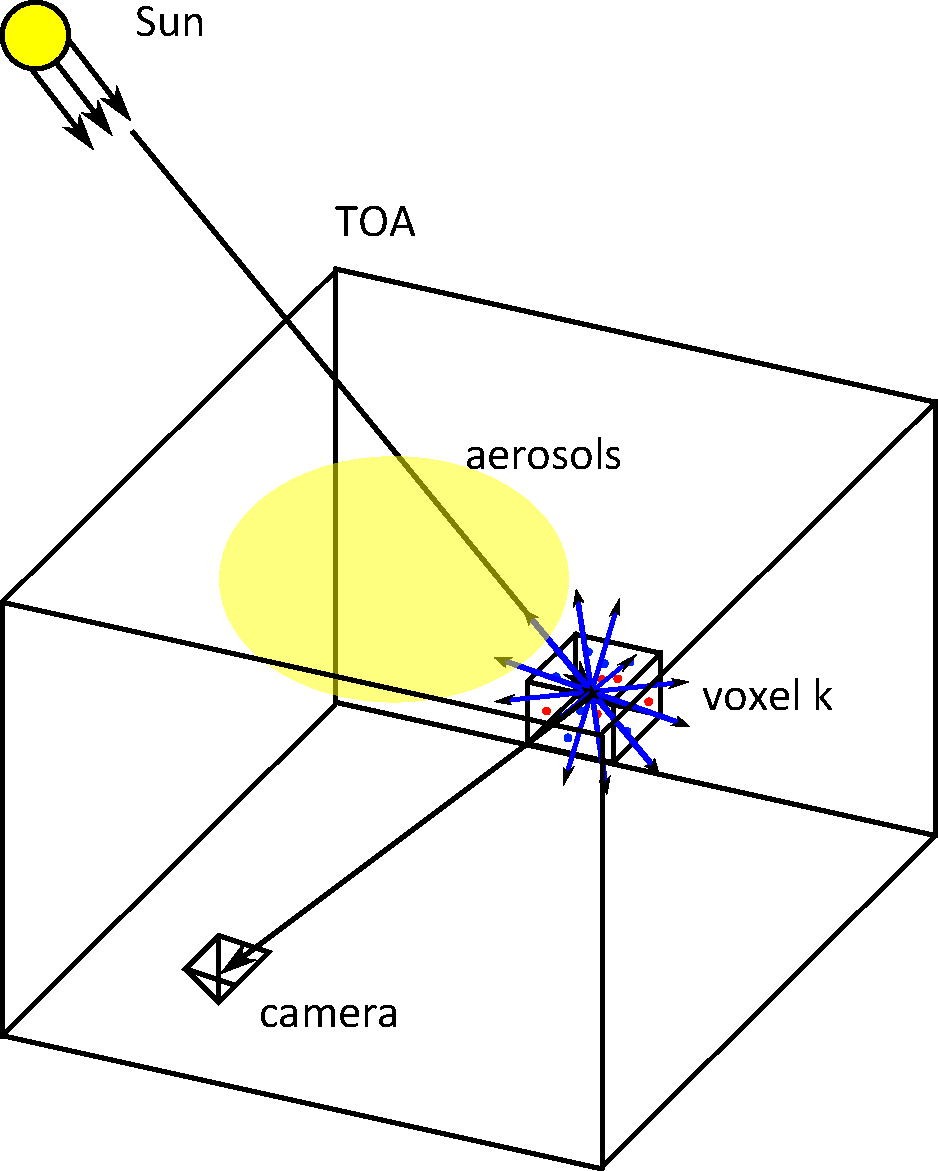
\includegraphics[width=\columnwidth]
          {images/atmo_settings3D11.pdf}}}
    \end{overprint}

  \end{columns}
\end{frame}

%%%%%%%%%%%%%%%%%%%%%%%%%%%%%%%%%%%%%%%%%%%%%%%%%%%%%%%

\begin{frame}[label=settings]{Simulation Settings}
  \begin{center}
    \begin{overlayarea}{\columnwidth}{8cm}
        \only<1>
        {\centerline{\includegraphics[width=\columnwidth]{images/voxels1.pdf}}}
        \only<2>
        {\centerline{\includegraphics[width=\columnwidth]{images/voxels2.pdf}}}
        \only<3>
        {\centerline{\includegraphics[width=\columnwidth]{images/voxels3.pdf}}}
        \only<4>
        {
          \hfill\hyperlink{air-density}{\beamergotobutton{Air Density}}  
          \centerline{\includegraphics[width=\columnwidth]{images/voxels4.pdf}}
        }
        \only<5>
        {
          \hfill\hyperlink{typical-concentrations}{\beamergotobutton{Aerosol Distribution}}  
          \centerline{\includegraphics[width=\columnwidth]{images/voxels5.pdf}}
          \begin{center}
            \tiny{Color represents aerosol density. The density units are $10^{6}~{\rm particles}/{\rm m}^3$}
          \end{center}
        }
    \end{overlayarea}
  \end{center}
\end{frame}

%%%%%%%%%%%%%%%%%%%%%%%%%%%%%%%%%%%%%%%%%%%%%%%%%%%%%%%

\begin{frame}{Synthesized Examples}
  \begin{columns}[C]
    \begin{column}{.7\textwidth}
      \begin{overlayarea}{\columnwidth}{8cm}
        \only<1>
        {\centerline{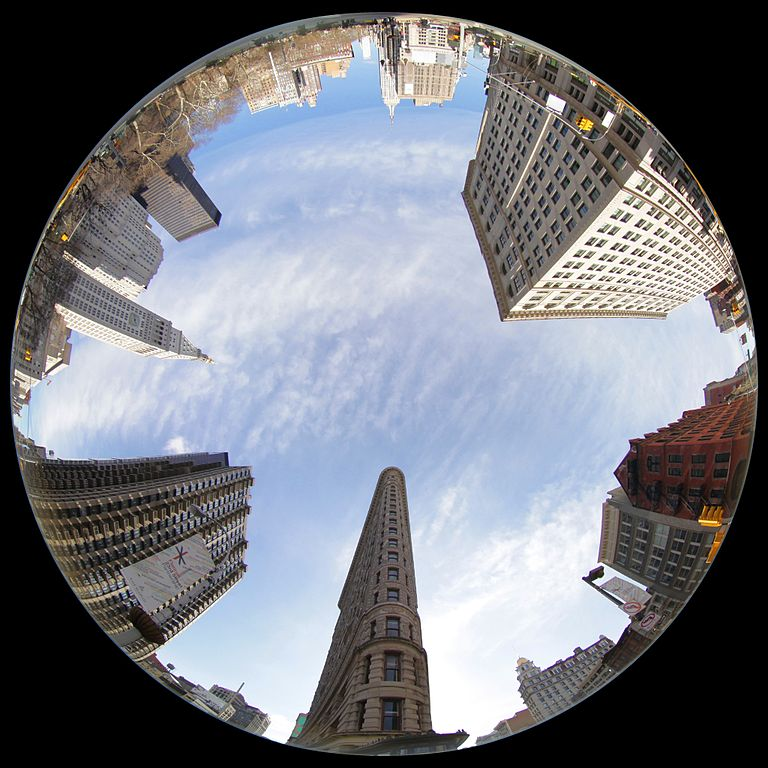
\includegraphics[height=7cm]{images/fisheye.jpg}}}
        \only<2>
        {\centerline{\includegraphics[height=7cm]{images/single_img1.pdf}}}
        \only<3>
        {\centerline{\includegraphics[height=7cm]{images/single_img2.pdf}}}
        \only<4>
        {\centerline{\includegraphics[height=7cm]{images/single_img3.pdf}}}
        \only<5>
        {\centerline{\includegraphics[height=7cm]{images/single_img4.pdf}}}
        \only<6>
        {\centerline{\includegraphics[height=7cm]{images/single_img5.pdf}}}
        \only<7>
        {\centerline{\includegraphics[height=7cm]{images/single_img6.pdf}}}
        \only<8>
        {\centerline{\includegraphics[height=7cm]{images/single_img7.pdf}}}
        \only<9>
        {\centerline{\includegraphics[height=7cm]{images/single_img8.pdf}}}
        \only<10>
        {\centerline{\includegraphics[height=7cm]{images/single_img9.pdf}}}
      \end{overlayarea}
    \end{column}
    \begin{column}{.3\textwidth}
      \begin{figure}
        \centering
        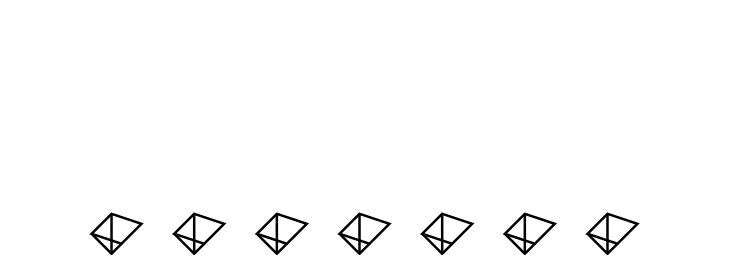
\includegraphics[width=\columnwidth]{images/atmo3d.pdf}
      \end{figure}
    \end{column}
  \end{columns}
\end{frame}

%%%%%%%%%%%%%%%%%%%%%%%%%%%%%%%%%%%%%%%%%%%%%%%%%%%%%%%

\subsection{Multi-Scattering Simulations}

\begin{frame}{Forward Simulated Models}
  \begin{columns}[C]
    \column{0.6\textwidth}
    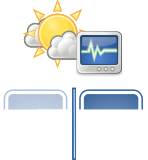
\includegraphics[width=\columnwidth]{images/diagram_models_multi.pdf}

    \column{0.4\textwidth}
    \begin{itemize}
    \item Physical
    \item Slow
    \item Not Analytic
    \item Joint work with Mr. Vadim Holodovsky
    \end{itemize}
  \end{columns}
\end{frame}

%%%

\begin{frame}{Monte Carlo Method}
  \begin{figure}
    \centering
    \begin{overprint}
      \only<1>
      {\centerline{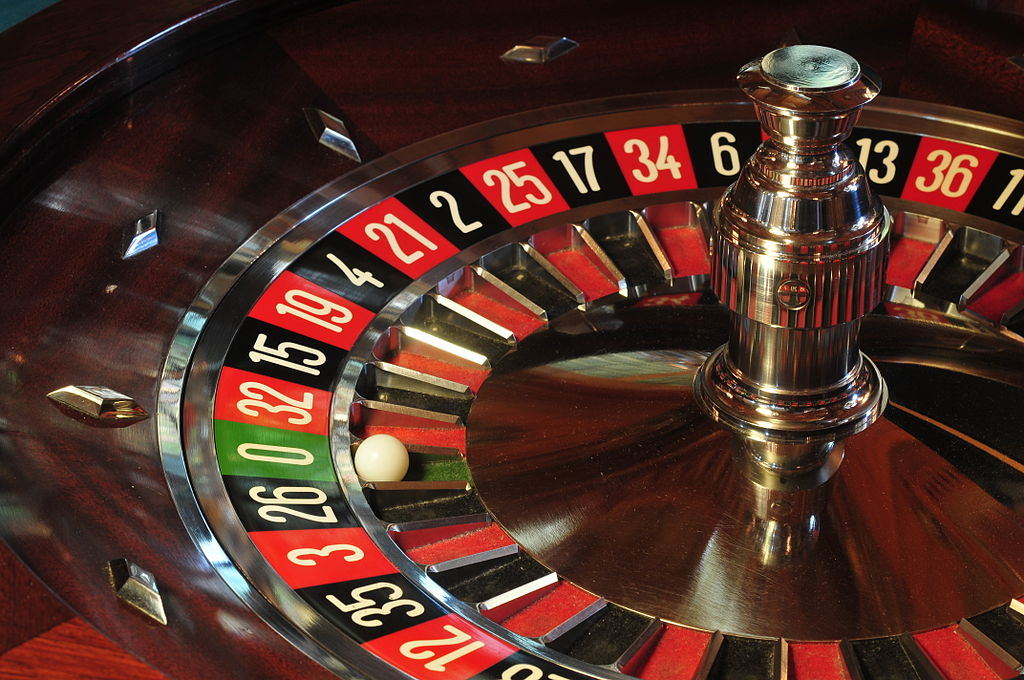
\includegraphics[height=7cm]{images/roullete.jpg}}} % Image taken from wikimedia commons 
      \only<2>
      {\centerline{\def\svgwidth{0.9\linewidth}\small{\input{images/mc_method1.pdf_tex}}}}
      \only<3>
      {\centerline{\def\svgwidth{0.9\linewidth}\small{\input{images/mc_method2.pdf_tex}}}}
      \only<4>
      {\centerline{\def\svgwidth{0.9\linewidth}\small{\input{images/mc_method3.pdf_tex}}}}
      \only<5>
      {\centerline{\def\svgwidth{0.9\linewidth}\small{\input{images/mc_method4.pdf_tex}}}}
      \only<6>
      {\centerline{\def\svgwidth{0.9\linewidth}\small{\input{images/mc_method5.pdf_tex}}}}
      \only<7>
      {\centerline{\def\svgwidth{0.9\linewidth}\small{\input{images/mc_method6.pdf_tex}}}}
      \only<8>
      {\centerline{\def\svgwidth{0.9\linewidth}\small{\input{images/mc_method7.pdf_tex}}}}
      \only<9>
      {\centerline{\def\svgwidth{0.9\linewidth}\small{\input{images/mc_method8.pdf_tex}}}}
      \only<10>
      {\centerline{\def\svgwidth{0.9\linewidth}\small{\input{images/mc_method9.pdf_tex}}}}
    \end{overprint}
  \end{figure}
\end{frame}

%%%

\begin{frame}{Monte Carlo Results}
  \begin{columns}[T]
    \begin{column}{.5\textwidth}
      \centering
      \only<1>
      {
        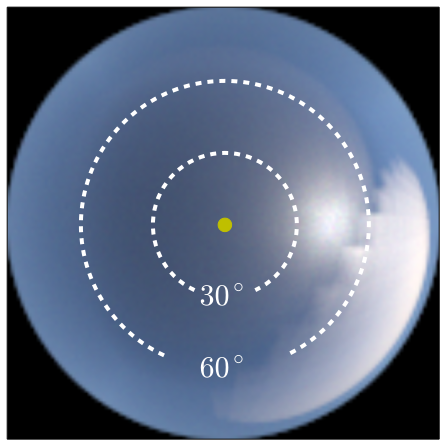
\includegraphics[height=0.60\textheight]{images/result_mc.pdf}
        \captionof{figure}{Monte Carlo Model\\{\color{red}$\sim 2$ Hour}}
      }
      \only<2>
      {
        \centerline{\def\svgwidth{0.8\linewidth}\footnotesize{\input{images/cross_section_x.pdf_tex}}}
        \captionof{figure}{X Cross Section}
      }
    \end{column}
    \begin{column}{.5\textwidth}
      \centering
      \only<1>
      {
        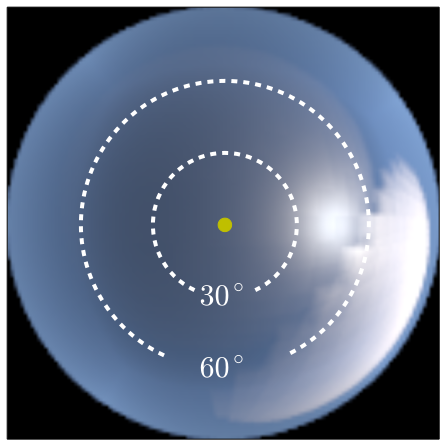
\includegraphics[height=0.60\textheight]{images/result_single.pdf}
        \captionof{figure}{Single Scattering Model\\{\color{red}$\sim 3$ Sec}}
      }
      \only<2>
      {
        \centerline{\def\svgwidth{0.8\linewidth}\footnotesize{\input{images/cross_section_y.pdf_tex}}}
        \captionof{figure}{Y Cross Section}
      }
    \end{column}
  \end{columns}
\end{frame}

%%%%%%%%%%%%%%%%%%%%%%%%%%%%%%%%%%%%%%%%%%%%%%%%%%%%%%%

\subsection{Inverse Problem}

\begin{frame}{Inverse Problem}
  \begin{center}
    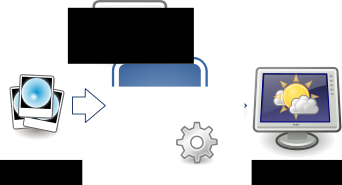
\includegraphics[height=5cm]{images/diagram_algorithm.pdf}
  \end{center}
\end{frame}

\begin{frame}{Multi-angle Tomographic Reconstruction}
  \begin{center}
    \centerline{\def\svgwidth{\linewidth}\small{\input{images/camera_network2.pdf_tex}}}
  \end{center}
\end{frame}

%%%%%%%%%%%%%%%%%%%%%%%%%%%%%%%%%%%%%%%%%%%%%%%%%%%%%%%

\subsubsection{Tomography}

\begin{frame}{Tomography}
  \begin{block}{}
    Reconstruct 3D object from its set of projections    
  \end{block}
\end{frame}

\begin{frame}{Attenuation Tomography}
  \begin{columns}
    \column{.5\textwidth}
    \includegraphics[height=6cm]{images/ct.png}
    \column{.5\textwidth}
    \includegraphics[height=5cm]{images/ct.jpg}
  \end{columns}  
  \begin{flushright}
    \only{\tiny http://medical-dictionary.thefreedictionary.com}
  \end{flushright}
  \only<2>
  {
    \CloudNote{0.4\textwidth}{0, 0}{
      Attenuation based \\
      Linear problem
    }
  }
\end{frame}

%%%%%%%%%%%%%%%%%%%%%%%%%%%%%%%%%%%%%%%%%%%%%%%%%%%%%%%

\begin{frame}{Emission Tomography}
  \begin{columns}
    \column{.5\textwidth}
    \begin{center}
      \includegraphics[width=\columnwidth]{images/tomography_emission.jpg}
      \captionof{figure}{\tiny Gregson at el. 2010}
    \end{center}
    \column{.5\textwidth}    
    \begin{center}
      \includegraphics[height=0.40\textheight]{gas.jpg}
      \captionof{figure}{\tiny Cosofret at el. 2009}
    \end{center}
  \end{columns}
  \only<2>
  {
    \CloudNote{0.4\textwidth}{0, 0}{
      No scattering \\
      Linear problem
    }
  }
\end{frame}

%%%%%%%%%%%%%%%%%%%%%%%%%%%%%%%%%%%%%%%%%%%%%%%%%%%%%%%

\begin{frame}{Optical Tomography}
  \begin{columns}[C]
    \begin{column}{.7\textwidth}
      \begin{itemize}
      \item Optical Tomography assumes a highly scattering medium
      \end{itemize}
    \end{column}
    \begin{column}{.3\textwidth}
      \centering
      \includegraphics[height=0.30\textheight]{Optical_Tomography.png}
    \end{column}
  \end{columns}  
  \only<2>
  {
    \CloudNote{0.4\textwidth}{0, 0}{
      Diffuse regime \\
      Controlled source
    }
  }
\end{frame}

%%%%%%%%%%%%%%%%%%%%%%%%%%%%%%%%%%%%%%%%%%%%%%%%%%%%%%%
 
\begin{frame}{Integral Imaging, Light-Field, Plenoptic}
  \begin{columns}[C]
    \begin{column}{.7\textwidth}
      \begin{itemize}
      \item Sample light in space and direction
      \item Enables re-focus, depth recovery, etc
      \end{itemize}
    \end{column}
    \begin{column}{.3\textwidth}
      \centering
      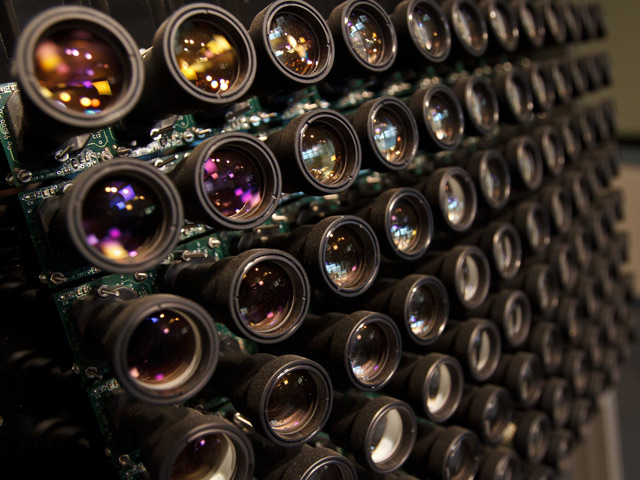
\includegraphics[height=0.30\textheight]{stanford_camera_array_640x480.jpg}
      \captionof{figure}{\tiny http://graphics.stanford.edu/}
      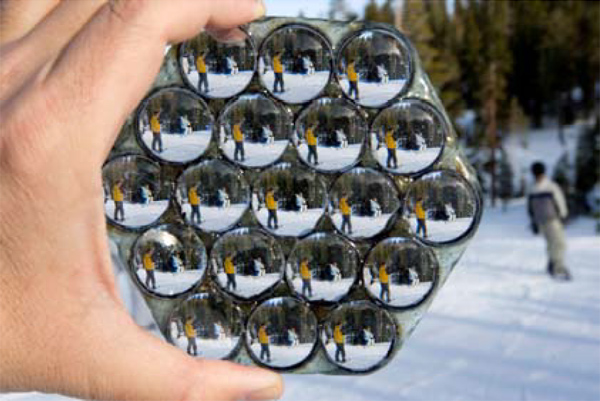
\includegraphics[height=0.30\textheight]{light-field-camera.jpg}
      \captionof{figure}{\tiny http://lightfield-forum.com}
    \end{column}
  \end{columns}
  \only<2>
  {
    \CloudNote{0.3\textwidth}{0, 0}{
      Small scale
    }
  }
\end{frame}

%%%%%%%%%%%%%%%%%%%%%%%%%%%%%%%%%%%%%%%%%%%%%%%%%%%%%%%

\begin{frame}{Multi-angle Tomographic Reconstruction}
  \only<1>
  {
    \begin{center}
      \centerline{\def\svgwidth{\linewidth}\small{\input{images/camera_network2.pdf_tex}}}
    \end{center}
  }
  \only<2>
  {
    \begin{block}{Objective Function}
      \begin{equation*}
        \CostFunc{\DistUnknown}
        = \sum_{c=1}^{N_{\rm views}}
        \left\| {\bm i}^{\rm measured}_c - {\bm i}_c ({\bm n})
        \right\|^2_2  + \eta \Psi ({\bm n})
      \end{equation*}
    \end{block}
  }
\end{frame}

%%%%%%%%%%%%%%%%%%%%%%%%%%%%%%%%%%%%%%%%%%%%%%%%%%%%%%%

\begin{frame}{Challenge}
  \begin{center}
    \centering
    \only<1>{\includegraphics[height=7cm]{images/challenge1.pdf}}
    \only<2>{\includegraphics[height=7cm]{images/challenge2.pdf}}
    \only<3>
    {
      \begin{enumerate}
      \item Prior Knowledge
      \item Large scale solvers
      \item Parallelize the algorithm
      \end{enumerate}
    }
  \end{center}
\end{frame}

%%%%%%%%%%%%%%%%%%%%%%%%%%%%%%%%%%%%%%%%%%%%%%%%%%%%%%%

\begin{frame}{Prior Knowledge}
  
  \begin{columns}
    \column{0.4\paperwidth}
    \begin{itemize}
    \item <2-> Known air distribution \tikz[na] \coordinate (known-air);
    \item <3-> \alert{Single known aerosol type} \tikz[na] \coordinate (known-part);
    \item <5-> Smoothness 
    \end{itemize}
    
    \column{0.45\paperwidth}
    \tikzstyle{background grid}=[draw, black!50,step=.5cm]
    \begin{tikzpicture}%[show background grid]
      % Put the graphic inside a node. This makes it easy to place the
      % graphic and to draw on top of it. 
      % The above right option is used to place the lower left corner
      % of the image at the (0,0) coordinate. 
      \onslide<4->{      
        \node [inner sep=0pt,above right] 
        {\centerline{\def\svgwidth{4cm}\input{images/challenge_only_n.pdf_tex}}};
      }

      % define destination coordinates
      \path (0.75, 2.25) coordinate (only-n-up)
            (0.75, 1.00) coordinate (only-n-down);
    \end{tikzpicture}

    % define overlays
    % Note the use of the overlay option. This is required when 
    % you want to access nodes in different pictures.
    \begin{tikzpicture}[overlay]
      \onslide<4->{
        \path[->,blue,thick] (known-air) edge [bend left] (only-n-up);
        \path[->,red,thick] (known-part) edge [bend right] (only-n-down);
      }
    \end{tikzpicture}
  \end{columns}
\end{frame}

%%%%%%%%%%%%%%%%%%%%%%%%%%%%%%%%%%%%%%%%%%%%%%%%%%%%%%%

\begin{frame}{Optimization}
  \begin{itemize}
  \item L-BFGS-B
    \begin{thebibliography}{blablabla}
    \bibitem[blablabla]{blablabla}
      R. H. Byrd, P. Lu and J. Nocedal.
      \newblock A Limited Memory Algorithm for Bound Constrained Optimization.
      \newblock {\em SIAM Journal on Scientific and Statistical Computing}, 1995.
    \end{thebibliography}
  \item Requires only the objective and its gradient
  \end{itemize}
\end{frame}

%%%%%%%%%%%%%%%%%%%%%%%%%%%%%%%%%%%%%%%%%%%%%%%%%%%%%%%

\begin{frame}[label=objective]{Optimization}
  \begin{block}{Objective Function}
    \begin{equation*}
      \only<1-5>{
        \CostFunc{\DistUnknown}
        = \sum_{c=1}^{N_{\rm views}}
        \left\|
          \tikz[baseline]{[\node[na] (d-im) {${\bm i}^{\rm measured}_c$};} - 
          \tikz[baseline]{[\node[na] (d-ie) {${\bm i}_c$};}
          \tikz[baseline]{[\node[na] (d-un1) {$({\bm n})$};}
        \right\|^2_2  + \eta \tikz[baseline]{ \node[na] (d2) {$\Psi$};}
        \tikz[baseline]{[\node[na] (d-un2) {$({\bm n})$};}
      }
      \only<6->
      {
        \CostFunc{\DistUnknown}
        = \sum_{c=1}^{N_{\rm views}}
        \left\|
          \tikz[baseline]{ \node[na] (d1) {$\MaskSun$};}[{\bm i}^{\rm measured}_c - {\bm i}_c({\bm n})]
        \right\|^2_2  + \eta \Psi ({\bm n})
      }
    \end{equation*}
  \end{block}
  \onslide<7>
  {
    \begin{block}{Estimated Aerosols}
      \begin{equation*}
        \DistEstimated =
        \argmin_{\DistUnknown \in \DistSet} \CostFunc{\DistUnknown}
      \end{equation*}
    \end{block}
  }
  \begin{tikzpicture}[overlay]
    \onslide<2>
    {
      \node[nodeyellow] at (4,1.5)(s1) {\hyperlink{ref-images}{Acquired Image}};
      \path[->] (s1) edge [bend right] (d-im);
    }
    \onslide<3>
    {
      \node[nodeyellow] at (8,1.5)(s2) {Estimated Image};
      \path[->] (s2) edge [bend left] (d-ie);
    }
    \onslide<4>
    {
      \node[nodered] at (6,1.5)(s3) {Unkown Aerosols Density};
      \path[->] (s3) edge [bend left] (d-un1);
      \path[->] (s3) edge [bend right] (d-un2);
    }
    \onslide<5>
    {
      \node[nodeblue] at (8,5.5)(s4) {\hyperlink{regularization}{Smoothness Constrain}};
      \path[->] (s4) edge [bend left] (d2);
    }
    \onslide<6>
    {
      \node[nodeblue] at (5,5.7) (s5) {\hyperlink{mask}{Multi-Scatter Mask}};
      \path[->] (s5) edge [bend right] (d1);
    }
  \end{tikzpicture}
\end{frame}

%%%%%%%%%%%%%%%%%%%%%%%%%%%%%%%%%%%%%%%%%%%%%%%%%%%%%%%

\begin{frame}[label=gradient]{Optimization}
  \only<1>
  {
    \begin{block}{Estimated Image}
      Inverse algorithm is based on the single-scattering model
     \begin{itemize}
      \item Fast
      \item Analytic $\Rightarrow$ differentiable
      \end{itemize}
      \begin{align*}
        {\bm i}_c= L^{\rm TOA} \OpCamera_c & \left[\tilde{\vect{\alpha}}^{\rm air}_c + \varpi^{\rm aerosol}\sigma^{\rm
              aerosol} P^{\rm aerosol}_g(\vect{\Phi}^{\rm scatter}_c) \odot{\bm
              n} \right] \odot \\
          & \exp\left[-(\vect{\tau}_c^{\rm air} + {\sigma}^{\rm aerosol}
            {\bm D}_c{\bm n})\right]
      \end{align*}
    \end{block}
  }
  \only<2>
  {
    \begin{block}{Gradient of the objective function}
      \begin{align*}
        \Grad{{\bm n}} E &= \\
        -&2\sum_{c=1}^{N_{\rm views}}
        \transpose{\left[\tikz[baseline]{\node[nodered] (d1) {${\bm J}_{{\bm i}_c}({\bm n})$};}\right]} \transpose{\MaskSun}\MaskSun[{\bm i}^{\rm
          measured}_c - {\bm i}_c({\bm n})] + 2 \eta
        \transpose{\Laplacian}\transpose{{\bf W}}{\bf W}\Laplacian{\bm n}
      \end{align*}
    \end{block}
  }
  \begin{tikzpicture}[overlay]
    \onslide<2>
    {
      \node[nodered] at (4,-.5)(s1) {\hyperlink{jacobian}{Jacobian}};
      \path[->] (s1) edge [bend right] (d1);
    }
  \end{tikzpicture}
\end{frame}

%%%%%%%%%%%%%%%%%%%%%%%%%%%%%%%%%%%%%%%%%%%%%%%%%%%%%%%

\begin{frame}{Parallelization} 
  \begin{columns}
    \column{0.8\textwidth}
    \begin{itemize}
    \item Processed using a computer cluster
    \item Each `camera' processed on a separate core
    \item Up to 100 cores = 100 simulated cameras
    \item A couple of hours to reconstruct 250K voxels
    \end{itemize}

    \column{0.2\textwidth}
    \begin{center}
      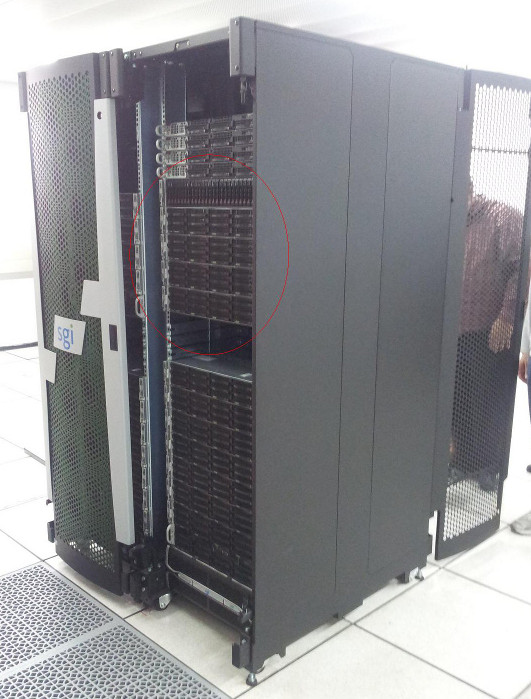
\includegraphics[width=\columnwidth]{tamnun.jpg}
    \end{center}
  \end{columns}
\end{frame}

%%%%%%%%%%%%%%%%%%%%%%%%%%%%%%%%%%%%%%%%%%%%%%%%%%%%%%%

\begin{frame}{Results - Original Atmospheres}
  \begin{center}
    \centerline{\def\svgwidth{1.15\linewidth}\footnotesize{\input{images/atmo3d_original.pdf_tex}}}
  \end{center}
  \begin{center}
    \tiny{Color represents aerosol density. The density units are $10^{6}~{\rm particles}/{\rm m}^3$}
  \end{center}
\end{frame}

%%%%%%%%%%%%%%%%%%%%%%%%%%%%%%%%%%%%%%%%%%%%%%%%%%%%%%%

\begin{frame}{Results - Single-scattering Simulations}
  \begin{center}
    \centerline{\def\svgwidth{1.15\linewidth}\footnotesize{\input{images/atmo3d_single.pdf_tex}}}
  \end{center}
  \begin{center}
    \tiny{Color represents aerosol density. The density units are $10^{6}~{\rm particles}/{\rm m}^3$}
  \end{center}
\end{frame}

%%%%%%%%%%%%%%%%%%%%%%%%%%%%%%%%%%%%%%%%%%%%%%%%%%%%%%%

\begin{frame}[label=results]{Results - Monte-Carlo Simulations}
  \begin{center}
    \centerline{\def\svgwidth{1.15\linewidth}\footnotesize{\input{images/atmo3d_mc.pdf_tex}}}
  \end{center}
  \begin{center}
    \tiny{Color represents aerosol density. The density units are $10^{6}~{\rm particles}/{\rm m}^3$}
    \hfill\hyperlink{error}{\beamergotobutton{Error}}
  \end{center}
\end{frame}

%%%%%%%%%%%%%%%%%%%%%%%%%%%%%%%%%%%%%%%%%%%%%%%%%%%%%%%%%%%%
%%%%%%%%%%%%%%%%%%%%%%%%%%%%%%%%%%%%%%%%%%%%%%%%%%%%%%%%%%%%

\section{Further Research Directions}

%%%%%%%%%%%%%%%%%%%%%%%%%%%%%%%%%%%%%%%%%%%%%%%%%%%%%%%

\subsection{Empirical Validation}

\begin{frame}{Experiment}
  \only<1>
  {
    \centering
    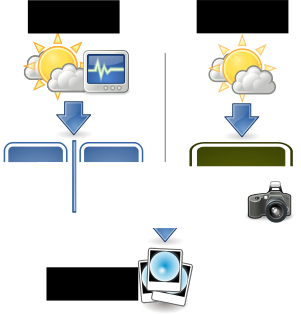
\includegraphics[height=7cm]{images/diagram_experiment2.pdf}    
  }
  \only<2>
  {
    \begin{columns}[C]
      \begin{column}{.7\textwidth}
        \begin{itemize}
        \item Grab multiple images from moving car
        \item Register images using GPS and/or SfM tools
        \item Collect ground truth
          \begin{itemize}
          \item MISR
          \item LIDAR
          \item AERONET
          \end{itemize}
        \end{itemize}
      \end{column}
      \begin{column}{.3\textwidth}
        \centering
        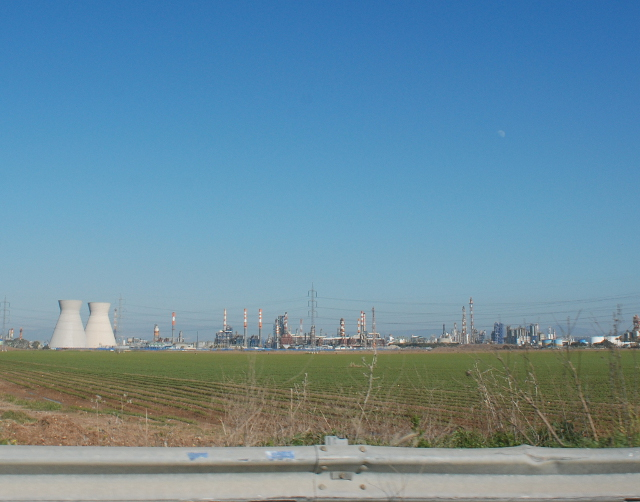
\includegraphics[height=0.30\textheight]{DSC_0688.JPG}\\
        \includegraphics[height=0.30\textheight]{AERONET.jpg}
        \captionof{figure}{\tiny http://earthobservatory.nasa.gov/}
      \end{column}
    \end{columns}
  }
\end{frame}

%%%%%%%%%%%%%%%%%%%%%%%%%%%%%%%%%%%%%%%%%%%%%%%%%%%%%%%

\subsection{Inverse Problem}

\begin{frame}{Algorithm Analysis}
  \begin{itemize}
  \item<1-> Limits:
    \begin{itemize}
    \item Validity of the Single Scattering approximation
    \item Theoretical reconstruction limits
    \end{itemize}
  \item<2-> Camera number vs Reconstruction resolution
  \item<3-> Implications of non uniform camera placement
  \end{itemize}
\end{frame}

%%%%%%%%%%%%%%%%%%%%%%%%%%%%%%%%%%%%%%%%%%%%%%%%%%%%%%%

\begin{frame}{Model Extension}
  \begin{itemize}
  \item<1-> Ground BRDF
  \item<2-> Unbounded Atmosphere
  \item<3-> Multiple particles
    \begin{itemize}
    \item Martonchik at el. 1998
    \end{itemize}
  \item<4-> Improve algorithm speed
  \item<5-> Higher scattering orders
  \item<6-> Cloudy Skies
  \end{itemize}
\end{frame}

%%%%%%%%%%%%%%%%%%%%%%%%%%%%%%%%%%%%%%%%%%%%%%%%%%%%%%%

\subsection{Aerosols in Partly Cloudy Skies}

\begin{frame}{Clouds}
  \begin{columns}[T]
    \begin{column}{.6\textwidth}
      \begin{itemize}
      \item High Optical Depth
        \begin{itemize}
        \item Single-Scattering approximation not-valid.
        \end{itemize}
      \item Affect radiation transfer:
        \begin{itemize}
        \item Cast shadows
        \item Reflect light
        \end{itemize}
      \end{itemize}
    \end{column}
    \begin{column}{.4\textwidth}
      \includegraphics[height=0.40\textheight]{clouds.jpg}
    \end{column}
  \end{columns}
\end{frame}

%%%%%%%%%%%%%%%%%%%%%%%%%%%%%%%%%%%%%%%%%%%%%%%%%%%%%%%

\begin{frame}{Reconstruction}

  \begin{itemize}
  \item Separate reconstruction
    \begin{itemize}
    \item SfM - Structure from Motion 
    \item Visual Hull
    \end{itemize}
  \item Add clouds to the forward model
  \end{itemize}

\end{frame}

%%%%%%%%%%%%%%%%%%%%%%%%%%%%%%%%%%%%%%%%%%%%%%%%%%%%%%%

\begin{frame}{}
  \includemedia[
  width=1.0\linewidth,height=0.66\linewidth,
  activate=pageopen,
  addresource=videos/cloudsnew.mp4,
  flashvars={source=videos/cloudsnew.mp4}
  ]{}{VPlayer.swf}
\end{frame}

%%%%%%%%%%%%%%%%%%%%%%%%%%%%%%%%%%%%%%%%%%%%%%%%%%%%%%%

\begin{frame}{}
  \begin{center}
    {\huge Thank You!}
  \end{center}
\end{frame}

%%%%%%%%%%%%%%%%%%%%%%%%%%%%%%%%%%%%%%%%%%%%%%%%%%%%%%%%%%%%
%%%%%%%%%%%%%%%%%%%%%% appendix %%%%%%%%%%%%%%%%%%%%%%%%%%%%
%%%%%%%%%%%%%%%%%%%%%%%%%%%%%%%%%%%%%%%%%%%%%%%%%%%%%%%%%%%%

\appendix

\begin{frame}[label=jacobian]{Jacobian (Differentiation)}
  \begin{block}{Jacobian Equation}
    \begin{align*}
      {\bm J}_{{\bm i}_c}({\bm n}) &= \\
      &L^{\rm TOA}{\sigma}^{\rm
        aerosol}({\bf A}-{\bf B}) \OpDiag{\exp[-(\vect{\tau}_c^{\rm air} +
        {\sigma}^{\rm aerosol} {\bm D}_c {\bm n})]}
      \transpose{\OpCamera_c}
    \end{align*}
    where
    \begin{align*}
      {\bf A} &= \varpi^{\rm aerosol}
      \OpDiag{ P_g^{\rm aerosol}(\vect{\Phi}^{\rm scatter}_c)} \\
      {\bf B} &= \transpose{{\bm D}_c}
      \OpDiag{[\tilde{\vect{\alpha}}^{\rm air}_c + \varpi^{\rm
          aerosol}\sigma^{\rm aerosol} P^{\rm aerosol}_g(\vect{\Phi}^{\rm
          scatter}_c) \odot{\bm n}    ]}
    \end{align*}
  \end{block}
  \hfill\hyperlink{gradient<2>}{\beamerreturnbutton{Return}}
\end{frame}

%%%%%%%%%%%%%%%%%%%%%%%%%%%%%%%%%%%%%%%%%%%%%%%%%%%%%%%

\begin{frame}[label=mask]{Multi-Scattering Mask}
  \begin{itemize}
  \item Weight error by Single-Scattering dominance
  \item Calculated empirically
  \end{itemize}
  \centerline{\includegraphics[height=4cm]{images/sun_mask.pdf}}
  \hfill\hyperlink{objective<6>}{\beamerreturnbutton{Return}} 
\end{frame}

%%%%%%%%%%%%%%%%%%%%%%%%%%%%%%%%%%%%%%%%%%%%%%%%%%%%%%%

\begin{frame}[label=regularization]{Regularization}
  \begin{itemize}
  \item Aerosol distributions are usually fuzzy
  \item 3D Laplacian enforces {\em smoothness}: $\Laplacian{\bm n} = \| \nabla^2{\bm  n}\|^2_2$
  \item Weighted by altitude: $w(k)=\exp\left[-h(k)/H^\mathrm{smooth}\right]$
  \item Regularization by $\Psi({\bm n}) = \| {\bf W} \Laplacian{\bm n}\|^2_2$
  \end{itemize}

  \hfill\hyperlink{objective<5>}{\beamerreturnbutton{Return}}
\end{frame}

%%%%%%%%%%%%%%%%%%%%%%%%%%%%%%%%%%%%%%%%%%%%%%%%%%%%%%%

\begin{frame}[label=ref-images]{Refernce Image}
  \begin{columns}[T]
    \begin{column}{.5\textwidth}
      \centering
        \includegraphics[height=0.60\textheight]{images/result_mc.pdf}
        \captionof{figure}{Monte Carlo Model}
    \end{column}
    \begin{column}{.5\textwidth}
      \centering
        \includegraphics[height=0.60\textheight]{images/result_single.pdf}
        \captionof{figure}{Single Scattering Model}
    \end{column}
  \end{columns}

  \hfill\hyperlink{objective<2>}{\beamerreturnbutton{Return}}
\end{frame}

%%%%%%%%%%%%%%%%%%%%%%%%%%%%%%%%%%%%%%%%%%%%%%%%%%%%%%%

\begin{frame}[label=aerosols-data]{Aerosols Info}
  \begin{center}
    \includegraphics<1>[width=\columnwidth]{images/aerosol_micrographs.jpg}
    \includegraphics<2>[height=7cm]{images/radiation_budget.jpg}
  \end{center}    
  \begin{flushright}
    \only<1> {\tiny http://earthobservatory.nasa.gov/Features/Aerosols/}
    \only<2> {\tiny http://calipsooutreach.hamptonu.edu/index.html}
  \end{flushright}
  \hfill\hyperlink{motivation}{\beamerreturnbutton{Return}}
\end{frame}

%%%%%%%%%%%%%%%%%%%%%%%%%%%%%%%%%%%%%%%%%%%%%%%%%%%%%%%

\begin{frame}[label=typical-concentrations]{Typical Aerosol Concentrations}
  \begin{center}
    \setlength{\tabcolsep}{5pt}
    \footnotesize
    \begin{tabular}{ l c c }
      \hline
      Atmosphere type & part./$m^3$ & Main radii $\mu m$ \\
      \hline
      Clean Country Air & $10^8$ & 0.1-1.0 \\[0.2cm]
      Pale blue haze, industr. & $10^{11}$ & 0.03-0.2 \\[0.2cm]
      Fog & $10^6$-$5 \times 10^7$ & 3-60 \\[0.2cm]
      Clouds, higher altitudes & $5 \times 10^7$-$1.5 \times 10^9$ & 2-30 \\
      \hline
    \end{tabular}
    \begin{flushright}
      {\tiny Source. Levi, Applied Optics, Volume 2}
     \end{flushright}
  \end{center}  
  \hfill\hyperlink{settings<5>}{\beamerreturnbutton{Return}}
\end{frame}

%%%%%%%%%%%%%%%%%%%%%%%%%%%%%%%%%%%%%%%%%%%%%%%%%%%%%%%

\begin{frame}[label=particle-type]{NASA - Component Particle Properties}
  \framezoom<1><2>[border](0cm,5.5cm)(7cm,0.71cm)
  \begin{center}
    \includegraphics[height=6.5cm]{images/particle_data.jpg}
  \end{center}    
  \hfill{\tiny Source. NASA}\hyperlink{settings<5>}{\beamerreturnbutton{Return}}
\end{frame}

%%%%%%%%%%%%%%%%%%%%%%%%%%%%%%%%%%%%%%%%%%%%%%%%%%%%%%%
\begin{frame}[label=air-density]{Atmosphere Density}
  \begin{center}
    \includegraphics[height=6.5cm]{images/vert_dist.jpg}
  \end{center}    
  \begin{flushright}
    {\tiny http://apollo.lsc.vsc.edu/}  \hyperlink{settings<4>}{\beamerreturnbutton{Return}}
  \end{flushright}
\end{frame}

%%%%%%%%%%%%%%%%%%%%%%%%%%%%%%%%%%%%%%%%%%%%%%%%%%%%%%%

\begin{frame}[label=tomo-algo]{Tomography Algorithms}
  \begin{block}{Filtered Back Projection}
    \only<1>{Linear projection is Radon transform}
    \only<2>{Invert using inverse Radon transform}
    \only<3>{Apply high pass filtering}
  \end{block}

  \begin{center}
    \includegraphics<1>[height=6.5cm]{images/radon.jpg}
    \includegraphics<2>[height=6.5cm]{images/radon_inv.jpg}
    \includegraphics<3>[height=6.5cm]{images/radon_inv_filt.jpg}
  \end{center}
\end{frame}

%%%%%%%%%%%%%%%%%%%%%%%%%%%%%%%%%%%%%%%%%%%%%%%%%%%%%%%

\begin{frame}{Tomography Algorithms}
  \begin{block}{ART - Algebraic Reconstruction Technique}
    Solve a set of linear equations of the form: \\
    \begin{equation*}
      \mat{A} \vect{x} = \vect{b}
    \end{equation*}
    using an iterative algorithm: \\
    \begin{equation*}
      \vect{x}^{k+1} = \vect{x}^{k} + \lambda_k \frac{b_{i} - \langle \vect{a}_{i}, \vect{x}^{k} \rangle}{\lVert \vect{a}_{i} \rVert^2} \vect{a}_{i}
    \end{equation*}
  \end{block}
\end{frame}

%%%%%%%%%%%%%%%%%%%%%%%%%%%%%%%%%%%%%%%%%%%%%%%%%%%%%%%

\begin{frame}[label=TOA]{TOA}
  \begin{center}
    \includegraphics<1>[height=5.5cm]{images/Solar_Spectrum.png}
    \only<2>
    {
      \begin{tabular}{l c c c}
        \hline
        \ & R & G & B \\
        \hline
        Wavelength  $[nm]$ & 672 & 558 & 446 \\[0.2cm]
        Intensity        & 255 & 237 & 224 \\
        \hline
      \end{tabular}
      \begin{flushright}
        \hyperlink{formation-model}{\beamerreturnbutton{Return}}
      \end{flushright}
    }
  \end{center}
\end{frame}

%%%%%%%%%%%%%%%%%%%%%%%%%%%%%%%%%%%%%%%%%%%%%%%%%%%%%%%

\begin{frame}[label=RTE]{Radiative Transfer Equation}
  \begin{align*}
    \hat{\Omega} \cdot \nabla I &+ (k_{s}+k_{a}) I_\nu = \\
    &j + \frac{1}{4\pi} \int_\Omega I \cdot P(\hat{\Omega},\Omega) d\Omega
  \end{align*}    
  \begin{flushright}
    \hyperlink{RT}{\beamerreturnbutton{Return}}
  \end{flushright}
\end{frame}

%%%%%%%%%%%%%%%%%%%%%%%%%%%%%%%%%%%%%%%%%%%%%%%%%%%%%%%

\begin{frame}[label=error]{Reconstruction error}
  \begin{center}
    \begin{tabular}{l c c}
      \hline
      \ & Clouds & Front \\
      \hline
      Single-Scat.  & 0.14 & 0.20 \\[0.2cm]
      Multi-Scat.   & 0.65 & 0.65 \\
      \hline
    \end{tabular}
    \begin{equation*}
      \epsilon=\frac{\|\hat{\bm n} - {\bm n}^{\rm true} \|_1}{\| {\bm n}^{\rm true} \|_1}
    \end{equation*}
    \begin{flushright}
      \hyperlink{results}{\beamerreturnbutton{Return}}
    \end{flushright}
  \end{center}
\end{frame}

% \begin{frame}{Common Atmospheric Models}
%   \begin{itemize}
%   \item<1> 1D or 2D models
%   \end{itemize}

%   \begin{center}
%     \includegraphics<1>[height=6cm]{images/atmosphere_layer.jpg}
%   \end{center}

%   \begin{flushright}
%     \only<1> {\tiny image taken from the Stratospheric Ozone Electronic Textbook}
%   \end{flushright}
% \end{frame}

%%%%%%%%%%%%%%%%%%%%%%%%%%%%%%%%%%%%%%%%%%%%%%%%%%%%%%%%%%%%
%%%%%%%%%%%%%%%%%%%%%%%% end %%%%%%%%%%%%%%%%%%%%%%%%%%%%%%%
%%%%%%%%%%%%%%%%%%%%%%%%%%%%%%%%%%%%%%%%%%%%%%%%%%%%%%%%%%%%

\end{document}

